%%
%% Automatically generated file from DocOnce source
%% (https://github.com/hplgit/doconce/)
%%
%%
% #ifdef PTEX2TEX_EXPLANATION
%%
%% The file follows the ptex2tex extended LaTeX format, see
%% ptex2tex: http://code.google.com/p/ptex2tex/
%%
%% Run
%%      ptex2tex myfile
%% or
%%      doconce ptex2tex myfile
%%
%% to turn myfile.p.tex into an ordinary LaTeX file myfile.tex.
%% (The ptex2tex program: http://code.google.com/p/ptex2tex)
%% Many preprocess options can be added to ptex2tex or doconce ptex2tex
%%
%%      ptex2tex -DMINTED myfile
%%      doconce ptex2tex myfile envir=minted
%%
%% ptex2tex will typeset code environments according to a global or local
%% .ptex2tex.cfg configure file. doconce ptex2tex will typeset code
%% according to options on the command line (just type doconce ptex2tex to
%% see examples). If doconce ptex2tex has envir=minted, it enables the
%% minted style without needing -DMINTED.
% #endif

% #define PREAMBLE

% #ifdef PREAMBLE
%-------------------- begin preamble ----------------------

\documentclass[%
oneside,                 % oneside: electronic viewing, twoside: printing
final,                   % or draft (marks overfull hboxes, figures with paths)
10pt]{article}

\listfiles               % print all files needed to compile this document

\usepackage{relsize,makeidx,color,setspace,amsmath,amsfonts}
\usepackage[table]{xcolor}
\usepackage{bm,microtype}

\usepackage[pdftex]{graphicx}

\usepackage{ptex2tex}
% #ifdef MINTED
\usepackage{minted}
\usemintedstyle{default}
% #endif

\usepackage[T1]{fontenc}
%\usepackage[latin1]{inputenc}
\usepackage{ucs}
\usepackage[utf8x]{inputenc}

\usepackage{lmodern}         % Latin Modern fonts derived from Computer Modern

% Hyperlinks in PDF:
\definecolor{linkcolor}{rgb}{0,0,0.4}
\usepackage{hyperref}
\hypersetup{
    breaklinks=true,
    colorlinks=true,
    linkcolor=linkcolor,
    urlcolor=linkcolor,
    citecolor=black,
    filecolor=black,
    %filecolor=blue,
    pdfmenubar=true,
    pdftoolbar=true,
    bookmarksdepth=3   % Uncomment (and tweak) for PDF bookmarks with more levels than the TOC
    }
%\hyperbaseurl{}   % hyperlinks are relative to this root

\setcounter{tocdepth}{2}  % number chapter, section, subsection

% Tricks for having figures close to where they are defined:
% 1. define less restrictive rules for where to put figures
\setcounter{topnumber}{2}
\setcounter{bottomnumber}{2}
\setcounter{totalnumber}{4}
\renewcommand{\topfraction}{0.85}
\renewcommand{\bottomfraction}{0.85}
\renewcommand{\textfraction}{0.15}
\renewcommand{\floatpagefraction}{0.7}
% 2. ensure all figures are flushed before next section
\usepackage[section]{placeins}
% 3. enable begin{figure}[H] (often leads to ugly pagebreaks)
%\usepackage{float}\restylefloat{figure}

% prevent orhpans and widows
\clubpenalty = 10000
\widowpenalty = 10000

\newenvironment{doconceexercise}{}{}
\newcounter{doconceexercisecounter}
% --- begin definition of \listofexercises command ---
\makeatletter
\newcommand\listofexercises{\section*{List of Exercises}
\@starttoc{loe}
}
\newcommand*{\l@doconceexercise}{\@dottedtocline{0}{0pt}{6.5em}}
\makeatother
% --- end definition of \listofexercises command ---



% ------ header in subexercises ------
%\newcommand{\subex}[1]{\paragraph{#1}}
%\newcommand{\subex}[1]{\par\vspace{1.7mm}\noindent{\bf #1}\ \ }
\makeatletter
% 1.5ex is the spacing above the header, 0.5em the spacing after subex title
\newcommand\subex{\@startsection{paragraph}{4}{\z@}%
                  {1.5ex\@plus1ex \@minus.2ex}%
                  {-0.5em}%
                  {\normalfont\normalsize\bfseries}}
\makeatother


% --- end of standard preamble for documents ---


% insert custom LaTeX commands...

\raggedbottom
\makeindex

%-------------------- end preamble ----------------------

\begin{document}

% endif for #ifdef PREAMBLE
% #endif


% ------------------- main content ----------------------



% ----------------- title -------------------------

\thispagestyle{empty}

\begin{center}
{\LARGE\bf
\begin{spacing}{1.25}
Infinite matter, from the electron gas to nuclear matter
\end{spacing}
}
\end{center}

% ----------------- author(s) -------------------------

\begin{center}
{\bf \href{{http://computationalphysics.no}}{Morten Hjorth-Jensen}, National Superconducting Cyclotron Laboratory and Department of Physics and Astronomy, Michigan State University, East Lansing, MI 48824, USA {\&} Department of Physics, University of Oslo, Oslo, Norway${}^{}$} \\ [0mm]
\end{center}

\begin{center}
% List of all institutions:
\end{center}
    
% ----------------- end author(s) -------------------------

\begin{center} % date
July 2015
\end{center}

\vspace{1cm}


\tableofcontents


\vspace{1cm} % after toc




\subsection{Introduction to studies of infinite matter}


Studies of infinite nuclear matter play an important role  in nuclear physics. The aim of this part of the lectures is to provide the necessary ingredients for perfoming studies of neutron star matter (or matter in $\beta$-equilibrium) and symmetric nuclear matter. We start however with the electron gas in two and three dimensions for both historical and pedagogical reasons. Since there are several benchmark calculations for the electron gas, this small detour will allow us to establish the necessary formalism. Thereafter we will study infinite nuclear matter 
\begin{itemize}
\item at the Hartree-Fock with realistic nuclear forces and

\item using many-body methods like coupled-cluster theory or in-medium SRG as discussed in our previous sections.
\end{itemize}

\noindent
\subsection{The infinite electron gas}

The electron gas is perhaps the only realistic model of a 
system of many interacting particles that allows for a solution
of the Hartree-Fock equations on a closed form. Furthermore, to first order in the interaction, one can also
compute on a closed form the total energy and several other properties of a many-particle systems. 
The model gives a very good approximation to the properties of valence electrons in metals.
The assumptions are

\begin{itemize}
 \item System of electrons that is not influenced by external forces except by an attraction provided by a uniform background of ions. These ions give rise to a uniform background charge. The ions are stationary.

 \item The system as a whole is neutral.

 \item We assume we have $N_e$ electrons in a cubic box of length $L$ and volume $\Omega=L^3$. This volume contains also a uniform distribution of positive charge with density $N_ee/\Omega$. 
\end{itemize}

\noindent
The homogeneous electron gas is one of the few examples of a system of many
interacting particles that allows for a solution of the mean-field
Hartree-Fock equations on a closed form.  To first order in the
electron-electron interaction, this applies to ground state properties
like the energy and its pertinent equation of state as well.  The
homogeneus electron gas is a system of electrons that is not
influenced by external forces except by an attraction provided by a
uniform background of ions. These ions give rise to a uniform
background charge.  The ions are stationary and the system as a whole
is neutral.
Irrespective of this simplicity, this system, in both two and
three-dimensions, has eluded a proper description of correlations in
terms of various first principle methods, except perhaps for quantum
Monte Carlo methods. In particular, the diffusion Monte Carlo
calculations of \href{{http://journals.aps.org/prl/abstract/10.1103/PhysRevLett.45.566}}{Ceperley} 
and \href{{http://journals.aps.org/prb/abstract/10.1103/PhysRevB.39.5005}}{Ceperley and Tanatar} 
are presently still considered as the
best possible benchmarks for the two- and three-dimensional electron
gas. 



The electron gas, in 
two or three dimensions is thus interesting as a test-bed for 
electron-electron correlations. The three-dimensional 
electron gas is particularly important as a cornerstone 
of the local-density approximation in density-functional 
theory. In the physical world, systems 
similar to the three-dimensional electron gas can be 
found in, for example, alkali metals and doped 
semiconductors. Two-dimensional electron fluids are 
observed on metal and liquid-helium surfaces, as well as 
at metal-oxide-semiconductor interfaces. However, the Coulomb 
interaction has an infinite range, and therefore 
long-range correlations play an essential role in the
electron gas. 




At low densities, the electrons become 
localized and form a lattice. This so-called Wigner 
crystallization is a direct consequence 
of the long-ranged repulsive interaction. At higher
densities, the electron gas is better described as a
liquid.
When using, for example, Monte Carlo methods the electron gas must be approximated 
by a finite system. The long-range Coulomb interaction 
in the electron gas causes additional finite-size effects  that are not
present in other infinite systems like nuclear matter or neutron star matter.
This poses additional challenges to many-body methods when applied 
to the electron gas.





\subsection{The infinite electron gas as a homogenous system}

This is a homogeneous system and the one-particle wave functions are given by plane wave functions normalized to a volume $\Omega$ 
for a box with length $L$ (the limit $L\rightarrow \infty$ is to be taken after we have computed various expectation values)
\[
\psi_{\mathbf{k}\sigma}(\mathbf{r})= \frac{1}{\sqrt{\Omega}}\exp{(i\mathbf{kr})}\xi_{\sigma}
\]
where $\mathbf{k}$ is the wave number and  $\xi_{\sigma}$ is a spin function for either spin up or down
\[ 
\xi_{\sigma=+1/2}=\left(\begin{array}{c} 1 \\ 0 \end{array}\right) \hspace{0.5cm}
\xi_{\sigma=-1/2}=\left(\begin{array}{c} 0 \\ 1 \end{array}\right).
\]




\subsection{Periodic boundary conditions}


We assume that we have periodic boundary conditions which limit the allowed wave numbers to
\[
k_i=\frac{2\pi n_i}{L}\hspace{0.5cm} i=x,y,z \hspace{0.5cm} n_i=0,\pm 1,\pm 2, \dots
\]
We assume first that the electrons interact via a central, symmetric and translationally invariant
interaction  $V(r_{12})$ with
$r_{12}=|\mathbf{r}_1-\mathbf{r}_2|$.  The interaction is spin independent.

The total Hamiltonian consists then of kinetic and potential energy
\[
\hat{H} = \hat{T}+\hat{V}.
\]
The operator for the kinetic energy can be written as
\[
\hat{T}=\sum_{\mathbf{k}\sigma}\frac{\hbar^2k^2}{2m}a_{\mathbf{k}\sigma}^{\dagger}a_{\mathbf{k}\sigma}.
\]



\subsection{Defining the Hamiltonian operator}

The Hamiltonian operator is given by
\[
\hat{H}=\hat{H}_{el}+\hat{H}_{b}+\hat{H}_{el-b},
\]
with the electronic part
\[
\hat{H}_{el}=\sum_{i=1}^N\frac{p_i^2}{2m}+\frac{e^2}{2}\sum_{i\ne j}\frac{e^{-\mu |\mathbf{r}_i-\mathbf{r}_j|}}{|\mathbf{r}_i-\mathbf{r}_j|},
\]
where we have introduced an explicit convergence factor
(the limit $\mu\rightarrow 0$ is performed after having calculated the various integrals).
Correspondingly, we have
\[
\hat{H}_{b}=\frac{e^2}{2}\int\int d\mathbf{r}d\mathbf{r}'\frac{n(\mathbf{r})n(\mathbf{r}')e^{-\mu |\mathbf{r}-\mathbf{r}'|}}{|\mathbf{r}-\mathbf{r}'|},
\]
which is the energy contribution from the positive background charge with density
$n(\mathbf{r})=N/\Omega$. Finally,
\[
\hat{H}_{el-b}=-\frac{e^2}{2}\sum_{i=1}^N\int d\mathbf{r}\frac{n(\mathbf{r})e^{-\mu |\mathbf{r}-\mathbf{x}_i|}}{|\mathbf{r}-\mathbf{x}_i|},
\]
is the interaction between the electrons and the positive background.



\subsection{Single-particle Hartree-Fock energy}

In the first exercise below we show that the Hartree-Fock energy can be written as 
\[
\varepsilon_{k}^{HF}=\frac{\hbar^{2}k^{2}}{2m_e}-\frac{e^{2}}
{\Omega^{2}}\sum_{k'\leq
k_{F}}\int d\mathbf{r}e^{i(\mathbf{k}'-\mathbf{k})\mathbf{r}}\int
d\mathbf{r'}\frac{e^{i(\mathbf{k}-\mathbf{k}')\mathbf{r}'}}
{\vert\mathbf{r}-\mathbf{r}'\vert}
\]
resulting in
\[
\varepsilon_{k}^{HF}=\frac{\hbar^{2}k^{2}}{2m_e}-\frac{e^{2}
k_{F}}{2\pi}
\left[
2+\frac{k_{F}^{2}-k^{2}}{kk_{F}}ln\left\vert\frac{k+k_{F}}
{k-k_{F}}\right\vert
\right]
\]



The previous result can be rewritten in terms of the density
\[
n= \frac{k_F^3}{3\pi^2}=\frac{3}{4\pi r_s^3},
\]
where $n=N_e/\Omega$, $N_e$ being the number of electrons, and $r_s$ is the radius of a sphere which represents the volum per conducting electron.  
It can be convenient to use the Bohr radius $a_0=\hbar^2/e^2m_e$.
For most metals we have a relation $r_s/a_0\sim 2-6$.  The quantity $r_s$ is dimensionless.


In the second exercise below  we find that
the total energy
$E_0/N_e=\langle\Phi_{0}|\hat{H}|\Phi_{0}\rangle/N_e$ for
for this system to first order in the interaction is given as 
\[
E_0/N_e=\frac{e^2}{2a_0}\left[\frac{2.21}{r_s^2}-\frac{0.916}{r_s}\right].
\]











% --- begin exercise ---
\begin{doconceexercise}
\refstepcounter{doconceexercisecounter}

\subsection*{Exercise \thedoconceexercisecounter: Hartree-Fock single-particle solution for the electron gas}


The electron gas model allows closed form solutions for quantities like the 
single-particle Hartree-Fock energy.  The latter quantity is given by the following expression
\[
\varepsilon_{k}^{HF}=\frac{\hbar^{2}k^{2}}{2m}-\frac{e^{2}}
{V^{2}}\sum_{k'\leq
k_{F}}\int d\mathbf{r}e^{i(\mathbf{k'}-\mathbf{k})\mathbf{r}}\int
d\mathbf{r}'\frac{e^{i(\mathbf{k}-\mathbf{k'})\mathbf{r}'}}
{\vert\mathbf{r}-\mathbf{r'}\vert}
\]


\subex{a)}
Show first that
\[
\varepsilon_{k}^{HF}=\frac{\hbar^{2}k^{2}}{2m}-\frac{e^{2}
k_{F}}{2\pi}
\left[
2+\frac{k_{F}^{2}-k^{2}}{kk_{F}}ln\left\vert\frac{k+k_{F}}
{k-k_{F}}\right\vert
\right]
\]

% --- begin hint in exercise ---

\paragraph{Hint.}
Hint: Introduce the convergence factor 
$e^{-\mu\vert\mathbf{r}-\mathbf{r}'\vert}$
in the potential and use  $\sum_{\mathbf{k}}\rightarrow
\frac{V}{(2\pi)^{3}}\int d\mathbf{k}$

% --- end hint in exercise ---


% --- begin solution of exercise ---
\paragraph{Solution.}
We want to show that, given the Hartree-Fock equation for the electron gas
\[
\varepsilon_{k}^{HF}=\frac{\hbar^{2}k^{2}}{2m}-\frac{e^{2}}
{V^{2}}\sum_{p\leq
k_{F}}\int d\mathbf{r}\exp{(i(\mathbf{p}-\mathbf{k})\mathbf{r})}\int
d\mathbf{r}'\frac{\exp{(i(\mathbf{k}-\mathbf{p})\mathbf{r}'})}
{\vert\mathbf{r}-\mathbf{r'}\vert}
\]
the single-particle energy can be written as
\[
\varepsilon_{k}^{HF}=\frac{\hbar^{2}k^{2}}{2m}-\frac{e^{2}
k_{F}}{2\pi}
\left[
2+\frac{k_{F}^{2}-k^{2}}{kk_{F}}ln\left\vert\frac{k+k_{F}}
{k-k_{F}}\right\vert
\right].
\]

We introduce the convergence factor 
$e^{-\mu\vert\mathbf{r}-\mathbf{r}'\vert}$
in the potential and use  $\sum_{\mathbf{k}}\rightarrow
\frac{V}{(2\pi)^{3}}\int d\mathbf{k}$. We can then rewrite the integral as 
\begin{align}
\frac{e^{2}}
{V^{2}}\sum_{k'\leq
k_{F}}\int d\mathbf{r}\exp{(i(\mathbf{k'}-\mathbf{k})\mathbf{r})}\int
d\mathbf{r}'\frac{\exp{(i(\mathbf{k}-\mathbf{p})\mathbf{r}'})}
{\vert\mathbf{r}-\mathbf{r'}\vert}= & \\
\frac{e^{2}}{V (2\pi)^3}  \int d\mathbf{r}\int
\frac{d\mathbf{r}'}{\vert\mathbf{r}-\mathbf{r'}\vert}\exp{(-i\mathbf{k}(\mathbf{r}-\mathbf{r}'))}\int d\mathbf{p}\exp{(i\mathbf{p}(\mathbf{r}-\mathbf{r}'))},
\end{align}
and introducing the abovementioned convergence factor we have
\begin{align}
\lim_{\mu \to 0}\frac{e^{2}}{V (2\pi)^3}  \int d\mathbf{r}\int d\mathbf{r}'\frac{\exp{(-\mu\vert\mathbf{r}-\mathbf{r}'\vert})}{\vert\mathbf{r}-\mathbf{r'}\vert}\int d\mathbf{p}\exp{(i(\mathbf{p}-\mathbf{k})(\mathbf{r}-\mathbf{r}'))}.
\end{align}


With a change variables to $\mathbf{x} = \mathbf{r}-\mathbf{r}'$ and $\mathbf{y}=\mathbf{r}'$ we rewrite the last integral as
\[
\lim_{\mu \to 0}\frac{e^{2}}{V (2\pi)^3}  \int d\mathbf{p}\int d\mathbf{y}\int d\mathbf{x}\exp{(i(\mathbf{p}-\mathbf{k})\mathbf{x})}\frac{\exp{(-\mu\vert\mathbf{x}\vert})}{\vert\mathbf{x}\vert}.
\]
The integration over $\mathbf{x}$ can be performed using spherical coordinates, resulting in (with $x=\vert \mathbf{x}\vert$)
\[
\int d\mathbf{x}\exp{(i(\mathbf{p}-\mathbf{k})\mathbf{x})}\frac{\exp{(-\mu\vert\mathbf{x}\vert})}{\vert\mathbf{x}\vert}=\int x^2 dx d\phi d\cos{(\theta)}\exp{(i(\mathbf{p}-\mathbf{k})x\cos{(\theta))}}\frac{\exp{(-\mu x)}}{x}.
\]


We obtain
\begin{align}
4\pi \int dx \frac{ \sin{(\vert \mathbf{p}-\mathbf{k}\vert)x} }{\vert \mathbf{p}-\mathbf{k}\vert}{\exp{(-\mu x)}}= \frac{4\pi}{\mu^2+\vert \mathbf{p}-\mathbf{k}\vert^2}.
\end{align}
This results gives us 
\begin{align}
\lim_{\mu \to 0}\frac{e^{2}}{V (2\pi)^3}  \int d\mathbf{p}\int d\mathbf{y}\frac{4\pi}{\mu^2+\vert \mathbf{p}-\mathbf{k}\vert^2}=\lim_{\mu \to 0}\frac{e^{2}}{ 2\pi^2}  \int d\mathbf{p}\frac{1}{\mu^2+\vert \mathbf{p}-\mathbf{k}\vert^2},
\end{align}
where we have used that the integrand on the left-hand side does not depend on $\mathbf{y}$ and that $\int d\mathbf{y}=V$.

Introducing spherical coordinates we can rewrite the integral as 
\begin{align}
\lim_{\mu \to 0}\frac{e^{2}}{ 2\pi^2}  \int d\mathbf{p}\frac{1}{\mu^2+\vert \mathbf{p}-\mathbf{k}\vert^2}=\frac{e^{2}}{ 2\pi^2}  \int d\mathbf{p}\frac{1}{\vert \mathbf{p}-\mathbf{k}\vert^2}=& \\
\frac{e^{2}}{\pi}  \int_0^{k_F} p^2dp\int_0^{\pi} d\theta\cos{(\theta)}\frac{1}{p^2+k^2-2pk\cos{(\theta)}},
\end{align}
and with the change of variables $\cos{(\theta)}=u$ we have 
\[
\frac{e^{2}}{\pi}  \int_0^{k_F} p^2dp\int_{0}^{\pi} d\theta\cos{(\theta)}\frac{1}{p^2+k^2-2pk\cos{(\theta)}}=\frac{e^{2}}{\pi}  \int_0^{k_F} p^2dp\int_{-1}^{1} du\frac{1}{p^2+k^2-2pku},
\]
which gives
\[
\frac{e^{2}}{k\pi}  \int_0^{k_F} pdp\left\{ln(\vert p+k\vert)-ln(\vert p-k\vert)\right\}.
\]

Introducing new variables $x=p+k$ and $y=p-k$, we obtain after some straightforward reordering of the integral
\[
\frac{e^{2}}{k\pi}\left[
kk_F+\frac{k_{F}^{2}-k^{2}}{kk_{F}}ln\left\vert\frac{k+k_{F}}
{k-k_{F}}\right\vert
\right],
\]
which gives the abovementioned expression for the single-particle energy.

% --- end solution of exercise ---

\subex{b)}
Rewrite the above result as a function of the density
\[
n= \frac{k_F^3}{3\pi^2}=\frac{3}{4\pi r_s^3},
\]
where $n=N/V$, $N$ being the number of particles, and $r_s$ is the radius of a sphere which represents the volum per conducting electron.


% --- begin solution of exercise ---
\paragraph{Solution.}
Introducing the dimensionless quantity $x=k/k_F$ and the function
\[
F(x) = \frac{1}{2}+\frac{1-x^2}{4x}\ln{\left\vert \frac{1+x}{1-x}\right\vert},
\]
we can rewrite the single-particle Hartree-Fock energy as 
\[
\varepsilon_{k}^{HF}=\frac{\hbar^{2}k^{2}}{2m}-\frac{2e^{2}
k_{F}}{\pi}F(k/k_F),
\]
and dividing by the non-interacting contribution at the Fermi level, 
\[
\varepsilon_{0}^{F}=\frac{\hbar^{2}k_F^{2}}{2m},
\]
we have
\[
\frac{\varepsilon_{k}^{HF} }{\varepsilon_{0}^{F}}=x^2-\frac{e^2m}{\hbar^2 k_F\pi}F(x)=x^2-\frac{4}{\pi k_Fa_0}F(x),
\]
where $a_0=0.0529$ nm is the Bohr radius, setting thereby a natural length scale. 


By introducing the radius $r_s$ of a sphere whose volume is the volume occupied by each electron, we can rewrite the previous equation in terms of $r_s$ using that the electron density $n=N/V$
\[
n=\frac{k_F^3}{3\pi^2} = \frac{3}{4\pi r_s^3},
\]
we have (with $k_F=1.92/r_s$,
\[
\frac{\varepsilon_{k}^{HF} }{\varepsilon_{0}^{F}}=x^2-\frac{e^2m}{\hbar^2 k_F\pi}F(x)=x^2-\frac{r_s}{a_0}0.663F(x),
\]
with $r_s \sim 2-6$ for most metals.

% --- end solution of exercise ---

It can be convenient to use the Bohr radius $a_0=\hbar^2/e^2m$.
For most metals we have a relation $r_s/a_0\sim 2-6$.

\subex{c)}
Make a plot of the free electron energy and the Hartree-Fock energy and discuss the behavior around the Fermi surface. Extract also   the Hartree-Fock band width $\Delta\varepsilon^{HF}$ defined as
\[ 
\Delta\varepsilon^{HF}=\varepsilon_{k_{F}}^{HF}-
\varepsilon_{0}^{HF}.
\]
Compare this results with the corresponding one for a free electron and comment your results. How large is the contribution due to the exchange term in the Hartree-Fock equation?


% --- begin solution of exercise ---
\paragraph{Solution.}
We can now define the so-called band gap, that is the scatter between the maximal and the minimal value of the electrons in the conductance band of a metal (up to the Fermi level). 
For $x=1$ and $r_s/a_0=4$ we have 
\[
\frac{\varepsilon_{k=k_F}^{HF} }{\varepsilon_{0}^{F}} = -0.326,
\]
and for $x=0$ we have
\[
\frac{\varepsilon_{k=0}^{HF} }{\varepsilon_{0}^{F}} = -2.652,
\]
which results in a gap at the Fermi level of 
\[
\Delta \varepsilon^{HF} = \frac{\varepsilon_{k=k_F}^{HF} }{\varepsilon_{0}^{F}}-\frac{\varepsilon_{k=0}^{HF} }{\varepsilon_{0}^{F}} = 2.326.
\]
This quantity measures the deviation from the $k=0$ single-particle energy and the energy at the Fermi level.
The general result is 
\[
\Delta \varepsilon^{HF} = 1+\frac{r_s}{a_0}0.663.
\]

The following python code produces a plot of the electron energy for a free electron (only kinetic energy) and 
for the Hartree-Fock solution. We have chosen here a ratio $r_s/a_0=4$ and the equations are plotted as funtions
of $k/f_F$. 
\bpycod
import numpy as np
from math import log
from  matplotlib import pyplot as plt
from matplotlib import rc, rcParams
import matplotlib.units as units
import matplotlib.ticker as ticker
rc('text',usetex=True)
rc('font',**{'family':'serif','serif':['Hartree-Fock energy']})
font = {'family' : 'serif',
        'color'  : 'darkred',
        'weight' : 'normal',
        'size'   : 16,
        }

N = 100
x = np.linspace(0.0, 2.0,N)
F = 0.5+np.log(abs((1.0+x)/(1.0-x)))*(1.0-x*x)*0.25/x
y = x*x -4.0*0.663*F

plt.plot(x, y, 'b-')
plt.plot(x, x*x, 'r-')
plt.title(r'{\bf Hartree-Fock single-particle energy for electron gas}', fontsize=20)     
plt.text(3, -40, r'Parameters: $r_s/a_0=4$', fontdict=font)
plt.xlabel(r'$k/k_F$',fontsize=20)
plt.ylabel(r'$\varepsilon_k^{HF}/\varepsilon_0^F$',fontsize=20)
# Tweak spacing to prevent clipping of ylabel
plt.subplots_adjust(left=0.15)
plt.savefig('hartreefockspelgas.pdf', format='pdf')
plt.show()
\epycod
From the plot we notice that the exchange term increases considerably the band gap
compared with the non-interacting gas of electrons.

% --- end solution of exercise ---
We will now define a quantity called the effective mass.
For $\vert\mathbf{k}\vert$ near $k_{F}$, we can Taylor expand the Hartree-Fock energy as  
\[
\varepsilon_{k}^{HF}=\varepsilon_{k_{F}}^{HF}+
\left(\frac{\partial\varepsilon_{k}^{HF}}{\partial k}\right)_{k_{F}}(k-k_{F})+\dots
\]
If we compare the latter with the corresponding expressiyon for the non-interacting system
\[
\varepsilon_{k}^{(0)}=\frac{\hbar^{2}k^{2}_{F}}{2m}+
\frac{\hbar^{2}k_{F}}{m}\left(k-k_{F}\right)+\dots ,
\]
we can define the so-called effective Hartree-Fock mass as
\[
m_{HF}^{*}\equiv\hbar^{2}k_{F}\left(
\frac{\partial\varepsilon_{k}^{HF}}
{\partial k}\right)_{k_{F}}^{-1}
\]
\subex{d)}
Compute $m_{HF}^{*}$ and comment your results.

\subex{e)}
Show that the level density (the number of single-electron states per unit energy) can be written as
\[
n(\varepsilon)=\frac{Vk^{2}}{2\pi^{2}}\left(
\frac{\partial\varepsilon}{\partial k}\right)^{-1}
\]
Calculate $n(\varepsilon_{F}^{HF})$ and comment the results.




\end{doconceexercise}
% --- end exercise ---




% --- begin exercise ---
\begin{doconceexercise}
\refstepcounter{doconceexercisecounter}

\subsection*{Exercise \thedoconceexercisecounter: Hartree-Fock ground state energy for the  electron gas in three dimensions}


We consider a system of electrons in infinite matter, the so-called electron gas. This is a homogeneous system and the one-particle states are given by plane wave function normalized to a volume $\Omega$ 
for a box with length $L$ (the limit $L\rightarrow \infty$ is to be taken after we have computed various expectation values)
\[
\psi_{\mathbf{k}\sigma}(\mathbf{r})= \frac{1}{\sqrt{\Omega}}\exp{(i\mathbf{kr})}\xi_{\sigma}
\]
where $\mathbf{k}$ is the wave number and  $\xi_{\sigma}$ is a spin function for either spin up or down
\[ 
\xi_{\sigma=+1/2}=\left(\begin{array}{c} 1 \\ 0 \end{array}\right) \hspace{0.5cm}
\xi_{\sigma=-1/2}=\left(\begin{array}{c} 0 \\ 1 \end{array}\right).
\]
We assume that we have periodic boundary conditions which limit the allowed wave numbers to
\[
k_i=\frac{2\pi n_i}{L}\hspace{0.5cm} i=x,y,z \hspace{0.5cm} n_i=0,\pm 1,\pm 2, \dots
\]
We assume first that the particles interact via a central, symmetric and translationally invariant
interaction  $V(r_{12})$ with
$r_{12}=|\mathbf{r}_1-\mathbf{r}_2|$.  The interaction is spin independent.

The total Hamiltonian consists then of kinetic and potential energy
\[
\hat{H} = \hat{T}+\hat{V}.
\]
The operator for the kinetic energy is given by
\[
\hat{T}=\sum_{\mathbf{k}\sigma}\frac{\hbar^2k^2}{2m}a_{\mathbf{k}\sigma}^{\dagger}a_{\mathbf{k}\sigma}.
\]


\subex{a)}
Find the expression for the interaction
$\hat{V}$ expressed with creation and annihilation operators.   The expression for the interaction
has to be written in  $k$ space, even though $V$ depends only on the relative distance. It means that you need to set up the Fourier transform $\langle \mathbf{k}_i\mathbf{k}_j| V | \mathbf{k}_m\mathbf{k}_n\rangle$.


% --- begin solution of exercise ---
\paragraph{Solution.}
A general two-body interaction element is given by (not using anti-symmetrized matrix elements)
\[ 
\hat{V} = \frac{1}{2} \sum_{pqrs} \langle pq \hat{v} \vert rs\rangle a_p^\dagger a_q^\dagger a_s a_r ,  
\]
where $\hat{v}$ is assumed to depend only on the relative distance between two interacting particles, that is
$\hat{v} = v(\vec r_1, \vec r_2) = v(|\vec r_1 - \vec r_2|) = v(r)$, with $r = |\vec r_1 - \vec r_2|$). 
In our case we have, writing out explicitely the spin degrees of freedom as well
\begin{equation}
\hat{V} = \frac{1}{2} \sum_{\substack{\sigma_p \sigma_q \\ \sigma_r \sigma_s}}
\sum_{\substack{\mathbf{k}_p \mathbf{k}_q \\ \mathbf{k}_r \mathbf{k}_s}}
\langle \mathbf{k}_p \sigma_p, \mathbf{k}_q \sigma_2\vert v \vert \mathbf{k}_r \sigma_3, \mathbf{k}_s \sigma_s\rangle
a_{\mathbf{k}_p \sigma_p}^\dagger a_{\mathbf{k}_q \sigma_q}^\dagger a_{\mathbf{k}_s \sigma_s} a_{\mathbf{k}_r \sigma_r} .
\label{eq:V_original}
\end{equation}

Inserting plane waves as eigenstates we can rewrite the matrix element as
\[ 
\langle \mathbf{k}_p \sigma_p, \mathbf{k}_q \sigma_q\vert \hat{v} \vert \mathbf{k}_r \sigma_r, \mathbf{k}_s \sigma_s\rangle =
\frac{1}{\Omega^2} \delta_{\sigma_p \sigma_r} \delta_{\sigma_q \sigma_s}
\int\int \exp{-i(\mathbf{k}_p \cdot \mathbf{r}_p)} \exp{-i( \mathbf{k}_q \cdot \mathbf{r}_q)} \hat{v}(r) \exp{i(\mathbf{k}_r \cdot \mathbf{r}_p)} \exp{i( \mathbf{k}_s \cdot \mathbf{r}_q)} d\mathbf{r}_p d\mathbf{r}_q , \]
where we have used the orthogonality properties of the spin functions. We change now the variables of integration
by defining $\mathbf{r} = \mathbf{r}_p - \mathbf{r}_q$, which gives $\mathbf{r}_p = \mathbf{r} + \mathbf{r}_q$ and $d^3 \mathbf{r} = d^3 \mathbf{r}_p$. 
The limits are not changed since they are from $-\infty$ to  $\infty$ for all integrals. This results in
\begin{align*}
\langle \mathbf{k}_p \sigma_p, \mathbf{k}_q \sigma_q\vert \hat{v} \vert \mathbf{k}_r \sigma_r, \mathbf{k}_s \sigma_s\rangle
&= \frac{1}{\Omega^2} \delta_{\sigma_p \sigma_r} \delta_{\sigma_q \sigma_s} \int
\exp{i (\mathbf{k}_s - \mathbf{k}_q) \cdot \mathbf{r}_q} \int v(r) \exp{i(\mathbf{k}_r - \mathbf{k}_p) \cdot ( \mathbf{r} + \mathbf{r}_q)} d\mathbf{r} d\mathbf{r}_q \\
&= \frac{1}{\Omega^2} \delta_{\sigma_p \sigma_r} \delta_{\sigma_q \sigma_s} \int v(r) \exp{i(\mathbf{k}_r - \mathbf{k}_p) \cdot \mathbf{r}}
\int \exp{i (\mathbf{k}_s - \mathbf{k}_q + \mathbf{k}_r - \mathbf{k}_p) \cdot \mathbf{r}_q} d\mathbf{r}_q d\mathbf{r} .
\end{align*}
We recognize the integral over $\mathbf{r}_q$ as a $\delta$-function, resulting in
\[ \langle \mathbf{k}_p \sigma_p, \mathbf{k}_q \sigma_q\vert \hat{v} \vert \mathbf{k}_r \sigma_r, \mathbf{k}_s \sigma_s\rangle =
\frac{1}{\Omega} \delta_{\sigma_p \sigma_r} \delta_{\sigma_q \sigma_s} \delta_{(\mathbf{k}_p + \mathbf{k}_q),(\mathbf{k}_r + \mathbf{k}_s)} \int v(r) \exp{i(\mathbf{k}_r - \mathbf{k}_p) \cdot \mathbf{r}} d^3r . \]
For this equation to be different from zero, we must have conservation of momenta, we need to satisfy
$\mathbf{k}_p + \mathbf{k}_q = \mathbf{k}_r + \mathbf{k}_s$. We can use the conservation of momenta to remove one of the summation variables in Eq. (\ref{eq:V_orginal}, resulting in
\[ \hat{V} =
\frac{1}{2\Omega} \sum_{\sigma \sigma'} \sum_{\mathbf{k}_p \mathbf{k}_q \mathbf{k}_r} \left[ \int v(r) \exp{i(\mathbf{k}_r - \mathbf{k}_p) \cdot \mathbf{r}} d^3r \right]
a_{\mathbf{k}_p \sigma}^\dagger a_{\mathbf{k}_q \sigma'}^\dagger a_{\mathbf{k}_p + \mathbf{k}_q - \mathbf{k}_r, \sigma'} a_{\mathbf{k}_r \sigma}, \]
which can be rewritten as 
\begin{equation}
\hat{V} =
\frac{1}{2\Omega} \sum_{\sigma \sigma'} \sum_{\mathbf{k} \mathbf{p} \mathbf{q}} \left[ \int v(r) \exp{-i( \mathbf{q} \cdot \mathbf{r})} d\mathbf{r} \right]
a_{\mathbf{k} + \mathbf{q}, \sigma}^\dagger a_{\mathbf{p} - \mathbf{q}, \sigma'}^\dagger a_{\mathbf{p} \sigma'} a_{\mathbf{k} \sigma},
\label{eq:V}
\end{equation}

This equation will be useful for our nuclear matter calculations as well. In the last equation we defined
the quantities
$\mathbf{p} = \mathbf{k}_p + \mathbf{k}_q - \mathbf{k}_r$, $\mathbf{k} = \mathbf{k}_r$ og $\mathbf{q} = \mathbf{k}_p - \mathbf{k}_r$.

% --- end solution of exercise ---

\subex{b)}
Calculate thereafter the reference energy for the infinite electron gas in three dimensions using the above expressions for the kinetic energy and the potential energy.


% --- begin solution of exercise ---
\paragraph{Solution.}
Let us now compute the expectation value of the reference energy using the expressions for the kinetic energy operator and the interaction.
We need to compute $\langle \Phi_0\vert \hat{H} \vert \Phi_0\rangle = \langle \Phi_0\vert \hat{T} \vert \Phi_0\rangle + \langle \Phi_0\vert \hat{V} \vert \Phi_0\rangle$, where $\vert \Phi_0\rangle$ is our reference Slater determinant, constructed from filling all single-particle states up to the Fermi level.
Let us start with the kinetic energy first
\[ \langle \Phi_0\vert \hat{T} \vert \Phi_0\rangle 
= \langle \Phi_0\vert \left( \sum_{\mathbf{p} \sigma} \frac{\hbar^2 p^2}{2m} a_{\mathbf{p} \sigma}^\dagger a_{\mathbf{p} \sigma} \right) \vert \Phi_0\rangle \\
= \sum_{\mathbf{p} \sigma} \frac{\hbar^2 p^2}{2m} \langle \Phi_0\rangle a_{\mathbf{p} \sigma}^\dagger a_{\mathbf{p} \sigma} \vert \Phi_0\rangle . \]
From the possible contractions using Wick's theorem, it is straightforward to convince oneself that the expression for the kinetic energy becomes
\[ \langle \Phi_0\vert \hat{T} \vert \Phi_0\rangle = \sum_{\mathbf{i} \leq F} \frac{\hbar^2 k_i^2}{m} = \frac{\Omega}{(2\pi)^3} \frac{\hbar^2}{m} \int_0^{k_F} k^2 d\mathbf{k}.
\]
The sum of the spin degrees of freedom results in  a factor of two only if we deal with identical spin $1/2$ fermions. 
Changing to spherical coordinates, the integral over the momenta $k$ results in the final expression
\[ \langle \Phi_0\vert \hat{T} \vert \Phi_0\rangle = \frac{\Omega}{(2\pi)^3} \left( 4\pi \int_0^{k_F} k^4 d\mathbf{k} \right) = \frac{4\pi\Omega}{(2\pi)^3} \frac{1}{5} k_F^5 = \frac{4\pi\Omega}{5(2\pi)^3} k_F^5 = \frac{\hbar^2 \Omega}{10\pi^2 m} k_F^5 . \]

The density of states in momentum space is given by $2\Omega/(2\pi)^3$, where we have included the degeneracy due to the spin degrees of freedom.
The volume is given by  $4\pi k_F^3/3$, and the number of particles becomes
\[ N = \frac{2\Omega}{(2\pi)^3} \frac{4}{3} \pi k_F^3 = \frac{\Omega}{3\pi^2} k_F^3 \quad \Rightarrow \quad
k_F = \left( \frac{3\pi^2 N}{\Omega} \right)^{1/3}. \]
This gives us
\begin{equation}
\langle \Phi_0\vert \hat{T} \vert \Phi_0\rangle =
\frac{\hbar^2 \Omega}{10\pi^2 m} \left( \frac{3\pi^2 N}{\Omega} \right)^{5/3} =
\frac{\hbar^2 (3\pi^2)^{5/3} N}{10\pi^2 m} \rho^{2/3} ,
\label{eq:T_forventning}
\end{equation}

We are now ready to calculate the expectation value of the potential energy
\begin{align*}
\langle \Phi_0\vert \hat{V} \vert \Phi_0\rangle 
&= \langle \Phi_0\vert \left( \frac{1}{2\Omega} \sum_{\sigma \sigma'} \sum_{\mathbf{k} \mathbf{p} \mathbf{q}} \left[ \int v(r) \exp{-i (\mathbf{q} \cdot \mathbf{r})} d\mathbf{r} \right]
a_{\mathbf{k} + \mathbf{q}, \sigma}^\dagger a_{\mathbf{p} - \mathbf{q}, \sigma'}^\dagger a_{\mathbf{p} \sigma'} a_{\mathbf{k} \sigma} \right) \vert \Phi_0\rangle \\
%
&= \frac{1}{2\Omega} \sum_{\sigma \sigma'} \sum_{\mathbf{k} \mathbf{p} \mathbf{q}} \left[ \int v(r) \exp{-i (\mathbf{q} \cdot \mathbf{r})} d\mathbf{r} \right]
\langle \Phi_0} a_{\mathbf{k} + \mathbf{q}, \sigma}^\dagger a_{\mathbf{p} - \mathbf{q}, \sigma'}^\dagger a_{\mathbf{p} \sigma'} a_{\mathbf{k} \sigma} \vert \Phi_0\rangle .
\end{align*}
The only contractions which result in non-zero results are those that involve states below the Fermi level, that is 
$k \leq k_F$, $p \leq k_F$, $|\mathbf{p} - \mathbf{q}| < \mathbf{k}_F$ and $|\mathbf{k} + \mathbf{q}| \leq k_F$. Due to momentum conservation we must also have $\mathbf{k} + \mathbf{q} = \mathbf{p}$, $\mathbf{p} - \mathbf{q} = \mathbf{k}$ and  $\sigma = \sigma'$ or  $\mathbf{k} + \mathbf{q} = \mathbf{k}$ and $\mathbf{p} - \mathbf{q} = \mathbf{p}$. 
Summarizing, we must have
\[ \mathbf{k} + \mathbf{q} = \mathbf{p} \quad \text{and} \quad \sigma = \sigma', \qquad
\text{or} \qquad
\mathbf{q} = \mathbf{0} . \]
We obtain then
\[ \langle \Phi_0\vert \hat{V} \vert \Phi_0\rangle =
\frac{1}{2\Omega} \left( \sum_{\sigma \sigma'} \sum_{\mathbf{i} \mathbf{j} \leq F} \left[ \int v(r) d\mathbf{r} \right] - \sum_{\sigma}
\sum_{\mathbf{i} \mathbf{j} \leq F} \left[ \int v(r) \exp{-i (\mathbf{k}_i \cdot \mathbf{r})} d\mathbf{r} \right] \right) , \]
which gives (and this applies to any potential which depends only on the relative distance between particles),
\begin{equation}
\langle \Phi_0\vert \hat{V} \vert \Phi_0\rangle =
\frac{1}{2\Omega} \left( N^2 \left[ \int v(r) d\mathbf{r} \right] - N \sum_{\mathbf{i} \leq F}} \left[ \int v(r) e^{-i \mathbf{k}_i\cdot \mathbf{r} d\mathbf{r} \right] \right) .
\label{eq:V_b}
\end{equation}

% --- end solution of exercise ---

The Hamiltonian operator is given by
\[
\hat{H}=\hat{H}_{el}+\hat{H}_{b}+\hat{H}_{el-b},
\]
with the electronic part
\[
\hat{H}_{el}=\sum_{i=1}^N\frac{p_i^2}{2m}+\frac{e^2}{2}\sum_{i\ne j}\frac{e^{-\mu |\mathbf{r}_i-\mathbf{r}_j|}}{|\mathbf{r}_i-\mathbf{r}_j|},
\]
where we have introduced an explicit convergence factor
(the limit $\mu\rightarrow 0$ is performed after having calculated the various integrals).
Correspondingly, we have
\[
\hat{H}_{b}=\frac{e^2}{2}\int\int d\mathbf{r}d\mathbf{r}'\frac{n(\mathbf{r})n(\mathbf{r}')e^{-\mu |\mathbf{r}-\mathbf{r}'|}}{|\mathbf{r}-\mathbf{r}'|},
\]
which is the energy contribution from the positive background charge with density
$n(\mathbf{r})=N/\Omega$. Finally,
\[
\hat{H}_{el-b}=-\frac{e^2}{2}\sum_{i=1}^N\int d\mathbf{r}\frac{n(\mathbf{r})e^{-\mu |\mathbf{r}-\mathbf{x}_i|}}{|\mathbf{r}-\mathbf{x}_i|},
\]
is the interaction between the electrons and the positive background.
\subex{c)}
Show that
\[
\hat{H}_{b}=\frac{e^2}{2}\frac{N^2}{\Omega}\frac{4\pi}{\mu^2},
\]
and
\[
\hat{H}_{el-b}=-e^2\frac{N^2}{\Omega}\frac{4\pi}{\mu^2}.
\]

\subex{d)}
Show thereafter that the final Hamiltonian can be written as 
\[
H=H_{0}+H_{I},
\]
with
\[
H_{0}={\displaystyle\sum_{\mathbf{k}\sigma}}
\frac{\hbar^{2}k^{2}}{2m}a_{\mathbf{k}\sigma}^{\dagger}
a_{\mathbf{k}\sigma},
\]
and
\[
H_{I}=\frac{e^{2}}{2\Omega}{\displaystyle\sum_{\sigma_{1}\sigma_{2}}}{\displaystyle\sum_{\mathbf{q}\neq 0,\mathbf{k},\mathbf{p}}}\frac{4\pi}{q^{2}}
a_{\mathbf{k}+\mathbf{q},\sigma_{1}}^{\dagger}
a_{\mathbf{p}-\mathbf{q},\sigma_{2}}^{\dagger}
a_{\mathbf{p}\sigma_{2}}a_{\mathbf{k}\sigma_{1}}.
\] 

\subex{e)}
Calculate $E_0/N=\langle \Phi_{0}\vert H\vert \Phi_{0}\rangle/N$ for for this system to first order in the interaction. Show that, by using
\[
\rho= \frac{k_F^3}{3\pi^2}=\frac{3}{4\pi r_0^3},
\]
with $\rho=N/\Omega$, $r_0$
being the radius of a sphere representing the volume an electron occupies 
and the Bohr radius $a_0=\hbar^2/e^2m$, 
that the energy per electron can be written as 
\[
E_0/N=\frac{e^2}{2a_0}\left[\frac{2.21}{r_s^2}-\frac{0.916}{r_s}\right].
\]
Here we have defined
$r_s=r_0/a_0$ to be a dimensionless quantity.

\subex{f)}
Plot your results. Why is this system stable?
Calculate thermodynamical quantities like the pressure, given by
\[
P=-\left(\frac{\partial E}{\partial \Omega}\right)_N,
\]
and the bulk modulus
\[
B=-\Omega\left(\frac{\partial P}{\partial \Omega}\right)_N,
\]
and comment your results.

We have to show first  that
\[
\hat{H}_{b}=\frac{e^2}{2}\frac{N_e^2}{\Omega}\frac{4\pi}{\mu^2},
\]
and
\[
\hat{H}_{el-b}=-e^2\frac{N_e^2}{\Omega}\frac{4\pi}{\mu^2}.
\]


And then that the final Hamiltonian can be written as 
\[
H=H_{0}+H_{I},
\]
with
\[
H_{0}={\displaystyle\sum_{\mathbf{k}\sigma}}
\frac{\hbar^{2}k^{2}}{2m_e}a_{\mathbf{k}\sigma}^{\dagger}
a_{\mathbf{k}\sigma},
\]
and
\[
H_{I}=\frac{e^{2}}{2\Omega}{\displaystyle\sum_{\sigma_{1}
\sigma_{2}}}{\displaystyle
\sum_{\mathbf{q}\neq 0,\mathbf{k},\mathbf{p}}}\frac{4\pi}{q^{2}}
a_{\mathbf{k}+\mathbf{q},\sigma_{1}}^{\dagger}
a_{\mathbf{p}-\mathbf{q},\sigma_{2}}^{\dagger}
a_{\mathbf{p}\sigma_{2}}a_{\mathbf{k}\sigma_{1}}.
\] 

Let us now calculate the following part of the Hamiltonian
\[ \hat H_b = \frac{e^2}{2} \iint \frac{n(\mathbf{r}) n(\mathbf{r}')e^{-\mu|\mathbf{r} - \mathbf{r}'|}}{|\mathbf{r} - \mathbf{r}'|} d\mathbf{r} d\mathbf{r}' , 
\]
where $n(\mathbf{r}) = N_e/\Omega$, the density of the positive background charge. We define $\mathbf{r}_{12} = \mathbf{r} - \mathbf{r}'$, resulting in $d\mathbf{r}_{12} = d\mathbf{r}$, and allowing us to rewrite the integral as
\[ 
\hat H_b = \frac{e^2 N_e^2}{2\Omega^2} \iint \frac{e^{-\mu |\mathbf{r}_{12}|}}{|\mathbf{r}_{12}|} d\mathbf{r}_{12} d\mathbf{r}' = \frac{e^2 N_e^2}{2\Omega} \int \frac{e^{-\mu |\mathbf{r}_{12}|}}{|\mathbf{r}_{12}|} d\mathbf{r}_{12} . 
\]
Here we have used that $\int \! \mathbf{r} = \Omega$. We change to spherical coordinates and the lack of angle 
dependencies yields a factor $4\pi$, resulting in
\[ 
\hat H_b = \frac{4\pi e^2 N_e^2}{2\Omega} \int_0^\infty re^{-\mu r} \, \mathrm{d} r . 
\]
Solving by partial integration
\[ \int_0^\infty re^{-\mu r} \, \mathrm{d} r = \left[ -\frac{r}{\mu} e^{-\mu r} \right]_0^\infty + \frac{1}{\mu} \int_0^\infty e^{-\mu r} \, \mathrm{d} r
= \frac{1}{\mu} \left[ - \frac{1}{\mu} e^{-\mu r} \right]_0^\infty = \frac{1}{\mu^2}, 
\]
gives
\[
\hat{H}_b = \frac{e^2}{2} \frac{N_e^2}{\Omega} \frac{4\pi}{\mu^2} .
\]
The next term is 
\[ 
\hat H_{el-b} = -e^2 \sum_{i = 1}^N \int \frac{n(\mathbf{r}) e^{-\mu |\mathbf{r} - \mathbf{x}_i|}}{|\mathbf{r} - \mathbf{x}_i|} \mathbf{r} . 
\]
Inserting  $n(\mathbf{r})$ and changing variables in the same way as in the previous integral $\mathbf{y} = \mathbf{r} - \mathbf{x}_i$, we get $\mathrm{d}^3 \mathbf{y} = \mathrm{d}^3 \mathbf{r}$. This gives
\begin{align}
\hat H_{el-b} = -\frac{e^2 N_e}{\Omega} \sum_{i = 1^N} \int \frac{e^{-\mu |\mathbf{y}|}}{|\mathbf{y}|} \, \mathrm{d}^3 \mathbf{y}
=  -\frac{4\pi e^2 N_e}{\Omega} \sum_{i = 1}^N \int_0^\infty y e^{-\mu y} \mathrm{d} y. 
\end{align}
We have already seen this  type of integral. The answer is 
\[ 
\hat H_{el-b} = -\frac{4\pi e^2 N_e}{\Omega} \sum_{i = 1}^N \frac{1}{\mu^2}, 
\]
which gives
\[
\hat H_{el-b} = -e^2 \frac{N_e^2}{\Omega} \frac{4\pi}{\mu^2} .
\]

Finally, we need to evaluate $\hat H_{el}$. This term reads
\[ 
\hat H_{el} = \sum_{i=1}^{N_e} \frac{\hat{\vec p}_i^2}{2m_e} + \frac{e^2}{2} \sum_{i \neq j} \frac{e^{-\mu |\mathbf{r}_i - \mathbf{r}_j|}}{\mathbf{r}_i - \mathbf{r}_j} . 
\]
The last term represents the repulsion between two electrons. It is a central symmetric interaction
and is translationally invariant. The potential is given by the expression
\[ 
v(|\mathbf{r}|) = e^2 \frac{e^{\mu|\mathbf{r}|}}{|\mathbf{r}|}, 
\]
which we derived in connection with the single-particle Hartree-Fock derivation.

More material will be added here!





\end{doconceexercise}
% --- end exercise ---


\subsection{Preparing the ground for numerical calculations; kinetic energy and Ewald term}

The kinetic energy operator is
\begin{align}
  \hat{H}_{\text{kin}} = -\frac{\hbar^{2}}{2m}\sum_{i=1}^{N}\nabla_{i}^{2},
\end{align}
where the sum is taken over all particles in the finite
box. The Ewald electron-electron interaction operator 
can be written as 
\begin{align}
  \hat{H}_{ee} = \sum_{i < j}^{N} v_{E}\left( \mathbf{r}_{i}-\mathbf{r}_{j}\right)
  + \frac{1}{2}Nv_{0},
\end{align}
where $v_{E}(\mathbf{r})$ is the effective two-body 
interaction and $v_{0}$ is the self-interaction, defined 
as $v_{0} = \lim_{\mathbf{r} \rightarrow 0} \left\{ v_{E}(\mathbf{r}) - 1/r\right\} $. 

The negative 
electron charges are neutralized by a positive, homogeneous 
background charge. Fraser \emph{et al.} explain how the
electron-background and background-background terms, 
$\hat{H}_{eb}$ and $\hat{H}_{bb}$, vanish
when using Ewald's interaction for the three-dimensional
electron gas. Using the same arguments, one can show that
these terms are also zero in the corresponding 
two-dimensional system. 




\subsection{Ewald correction term}

In the three-dimensional electron gas, the Ewald 
interaction is 
\begin{align}
  v_{E}(\mathbf{r}) &= \sum_{\mathbf{k} \neq \mathbf{0}}
  \frac{4\pi }{L^{3}k^{2}}e^{i\mathbf{k}\cdot \mathbf{r}}
  e^{-\eta^{2}k^{2}/4} \nonumber \\
  &+ \sum_{\mathbf{R}}\frac{1}{\left| \mathbf{r}
    -\mathbf{R}\right| } \mathrm{erfc} \left( \frac{\left| 
    \mathbf{r}-\mathbf{R}\right|}{\eta }\right)
  - \frac{\pi \eta^{2}}{L^{3}},
\end{align}
where $L$ is the box side length, $\mathrm{erfc}(x)$ is the 
complementary error function, and $\eta $ is a free
parameter that can take any value in the interval 
$(0, \infty )$.



\subsection{Interaction in momentum space}

The translational vector 
\begin{align}
  \mathbf{R} = L\left(n_{x}\mathbf{u}_{x} + n_{y}
  \mathbf{u}_{y} + n_{z}\mathbf{u}_{z}\right) ,
\end{align}
where $\mathbf{u}_{i}$ is the unit vector for dimension $i$,
is defined for all integers $n_{x}$, $n_{y}$, and 
$n_{z}$. These vectors are used to obtain all image
cells in the entire real space. 
The parameter $\eta $ decides how 
the Coulomb interaction is divided into a short-ranged
and long-ranged part, and does not alter the total
function. However, the number of operations needed
to calculate the Ewald interaction with a desired 
accuracy depends on $\eta $, and $\eta $ is therefore 
often chosen to optimize the convergence as a function
of the simulation-cell size. In
our calculations, we choose $\eta $ to be an infinitesimally
small positive number, similarly as was done by \href{{https://journals.aps.org/prb/abstract/10.1103/PhysRevB.86.035111}}{Shepherd *et al.*} and \href{{https://journals.aps.org/prb/abstract/10.1103/PhysRevB.88.115138}}{Roggero *et al.*}.

This gives an interaction that is evaluated only in
Fourier space. 

When studying the two-dimensional electron gas, we
use an Ewald interaction that is quasi two-dimensional.
The interaction is derived in three dimensions, with 
Fourier discretization in only two dimensions. The Ewald effective
interaction has the form 
\begin{align}
  v_{E}(\mathbf{r}) &= \sum_{\mathbf{k} \neq \mathbf{0}} 
  \frac{\pi }{L^{2}k}\left\{ e^{-kz} \mathrm{erfc} \left(
  \frac{\eta k}{2} - \frac{z}{\eta }\right)+ \right. \nonumber \\
  & \left. e^{kz}\mathrm{erfc} \left( \frac{\eta k}{2} + \frac{z}{\eta }
  \right) \right\} e^{i\mathbf{k}\cdot \mathbf{r}_{xy}} 
  \nonumber \\
  & + \sum_{\mathbf{R}}\frac{1}{\left| \mathbf{r}-\mathbf{R}
    \right| } \mathrm{erfc} \left( \frac{\left| \mathbf{r}-\mathbf{R}
    \right|}{\eta }\right) \nonumber \\
  & - \frac{2\pi}{L^{2}}\left\{ z\mathrm{erf} \left( \frac{z}{\eta }
  \right) + \frac{\eta }{\sqrt{\pi }}e^{-z^{2}/\eta^{2}}\right\},
\end{align}
where the Fourier vectors $\mathbf{k}$ and the position vector
$\mathbf{r}_{xy}$ are defined in the $(x,y)$ plane. When
applying the interaction $v_{E}(\mathbf{r})$ to two-dimensional
systems, we set $z$ to zero. 


Similarly as in the 
three-dimensional case, also here we 
choose $\eta $ to approach zero from above. The resulting 
Fourier-transformed interaction is
\begin{align}
  v_{E}^{\eta = 0, z = 0}(\mathbf{r}) = \sum_{\mathbf{k} \neq \mathbf{0}} 
  \frac{2\pi }{L^{2}k}e^{i\mathbf{k}\cdot \mathbf{r}_{xy}}. 
\end{align}
The self-interaction $v_{0}$ is a constant that can be 
included in the reference energy.




\subsection{Antisymmetrized matrix elements in three dimensions}

In the three-dimensional electron gas, the antisymmetrized
matrix elements are
\begin{align} \label{eq:vmat_3dheg}
  & \langle \mathbf{k}_{p}m_{s_{p}}\mathbf{k}_{q}m_{s_{q}}
  |\tilde{v}|\mathbf{k}_{r}m_{s_{r}}\mathbf{k}_{s}m_{s_{s}}\rangle_{AS} 
  \nonumber \\
  & = \frac{4\pi }{L^{3}}\delta_{\mathbf{k}_{p}+\mathbf{k}_{q},
    \mathbf{k}_{r}+\mathbf{k}_{s}}\left\{ 
  \delta_{m_{s_{p}}m_{s_{r}}}\delta_{m_{s_{q}}m_{s_{s}}}
  \left( 1 - \delta_{\mathbf{k}_{p}\mathbf{k}_{r}}\right) 
  \frac{1}{|\mathbf{k}_{r}-\mathbf{k}_{p}|^{2}}
  \right. \nonumber \\
  & \left. - \delta_{m_{s_{p}}m_{s_{s}}}\delta_{m_{s_{q}}m_{s_{r}}}
  \left( 1 - \delta_{\mathbf{k}_{p}\mathbf{k}_{s}} \right)
  \frac{1}{|\mathbf{k}_{s}-\mathbf{k}_{p}|^{2}} 
  \right\} ,
\end{align}
where the Kronecker delta functions 
$\delta_{\mathbf{k}_{p}\mathbf{k}_{r}}$ and
$\delta_{\mathbf{k}_{p}\mathbf{k}_{s}}$ ensure that the 
contribution with zero momentum transfer vanishes.


Similarly, the matrix elements for the two-dimensional
electron gas are
\begin{align} \label{eq:vmat_2dheg}
  & \langle \mathbf{k}_{p}m_{s_{p}}\mathbf{k}_{q}m_{s_{q}}
  |v|\mathbf{k}_{r}m_{s_{r}}\mathbf{k}_{s}m_{s_{s}}\rangle_{AS} 
  \nonumber \\
  & = \frac{2\pi }{L^{2}}
  \delta_{\mathbf{k}_{p}+\mathbf{k}_{q},\mathbf{k}_{r}+\mathbf{k}_{s}}
  \left\{ \delta_{m_{s_{p}}m_{s_{r}}}\delta_{m_{s_{q}}m_{s_{s}}} 
  \left( 1 - \delta_{\mathbf{k}_{p}\mathbf{k}_{r}}\right)
  \frac{1}{
    |\mathbf{k}_{r}-\mathbf{k}_{p}|} \right.
  \nonumber \\
  & - \left. \delta_{m_{s_{p}}m_{s_{s}}}\delta_{m_{s_{q}}m_{s_{r}}}
  \left( 1 - \delta_{\mathbf{k}_{p}\mathbf{k}_{s}}\right)
  \frac{1}{ 
    |\mathbf{k}_{s}-\mathbf{k}_{p}|}
  \right\} ,
\end{align}
where the single-particle momentum vectors $\mathbf{k}_{p,q,r,s}$
are now defined in two dimensions.

In actual  calculations, the 
single-particle energies, defined by the operator $\hat{f}$, are given by
\begin{align}
  \langle \mathbf{k}_{p}|f|\mathbf{k}_{q} \rangle
  = \frac{\hbar^{2}k_{p}^{2}}{2m}\delta_{\mathbf{k}_{p},
  \mathbf{k}_{q}} + \sum_{\mathbf{k}_{i}}\langle 
  \mathbf{k}_{p}\mathbf{k}_{i}|v|\mathbf{k}_{q}
  \mathbf{k}_{i}\rangle_{AS}.
  \label{eq:fock_heg}
\end{align}



\subsection{Periodic boundary conditions and single-particle states}

When using periodic boundary conditions, the 
discrete-momentum single-particle basis functions 
\[
\phi_{\mathbf{k}}(\mathbf{r}) =
e^{i\mathbf{k}\cdot \mathbf{r}}/L^{d/2}
\]
are associated with 
the single-particle energy   
\begin{align}
  \varepsilon_{n_{x}, n_{y}} = \frac{\hbar^{2}}{2m} \left( \frac{2\pi }{L}\right)^{2}\left( n_{x}^{2} + n_{y}^{2}\right)
\end{align}
for two-dimensional sytems and 
\begin{align}
  \varepsilon_{n_{x}, n_{y}, n_{z}} = \frac{\hbar^{2}}{2m}
  \left( \frac{2\pi }{L}\right)^{2}
  \left( n_{x}^{2} + n_{y}^{2} + n_{z}^{2}\right)
\end{align} 
for three-dimensional systems.


We choose  the single-particle basis such that both the occupied and 
unoccupied single-particle spaces have a closed-shell 
structure. This means that all single-particle states 
corresponding to energies below a chosen cutoff are
included in the basis. We study only the unpolarized spin
phase, in which all orbitals are occupied with one spin-up 
and one spin-down electron. 


The table illustrates  how single-particle energies
    fill energy shells in a two-dimensional electron box.
  Here $n_{x}$ and $n_{y}$ are the momentum quantum numbers,
  $n_{x}^{2} + n_{y}^{2}$ determines the single-particle 
  energy level, $N_{\uparrow \downarrow }$ represents the 
  cumulated number of spin-orbitals in an unpolarized spin
  phase, and $N_{\uparrow \uparrow }$ stands for the
  cumulated number of spin-orbitals in a spin-polarized
  system.




\subsection{Magic numbers for the two-dimensional electron gas}



\begin{quote}
\begin{tabular}{ccccc}
\hline
\multicolumn{1}{c}{ $n_{x}^{2}+n_{y}^{2}$ } & \multicolumn{1}{c}{ $n_{x}$ } & \multicolumn{1}{c}{ $n_{y}$ } & \multicolumn{1}{c}{ $N_{\uparrow \downarrow }$ } & \multicolumn{1}{c}{ $N_{\uparrow \uparrow }$ } \\
\hline
0                     & 0       & 0       & 2                          & 1                        \\
\hline
1                     & -1      & 0       &                            &                          \\
                      & 1       & 0       &                            &                          \\
                      & 0       & -1      &                            &                          \\
                      & 0       & 1       & 10                         & 5                        \\
\hline
2                     & -1      & -1      &                            &                          \\
                      & -1      & 1       &                            &                          \\
                      & 1       & -1      &                            &                          \\
                      & 1       & 1       & 18                         & 9                        \\
\hline
4                     & -2      & 0       &                            &                          \\
                      & 2       & 0       &                            &                          \\
                      & 0       & -2      &                            &                          \\
                      & 0       & 2       & 26                         & 13                       \\
\hline
5                     & -2      & -1      &                            &                          \\
                      & 2       & -1      &                            &                          \\
                      & -2      & 1       &                            &                          \\
                      & 2       & 1       &                            &                          \\
                      & -1      & -2      &                            &                          \\
                      & -1      & 2       &                            &                          \\
                      & 1       & -2      &                            &                          \\
                      & 1       & 2       & 42                         & 21                       \\
\hline
\end{tabular}
\end{quote}

\noindent
\subsection{Hartree-Fock energies}

Finally, a useful benchmark for our calculations is the expression for
the reference energy $E_0$ per particle.
Defining the $T=0$ density $\rho_0$, we can in turn determine in three
dimensions the radius $r_0$ of a sphere representing the volume an
electron occupies (the classical electron radius) as
\[
r_0= \left(\frac{3}{4\pi \rho}\right)^{1/3}.
\]
In two dimensions the corresponding quantity is
\[
r_0= \left(\frac{1}{\pi \rho}\right)^{1/2}.
\]


One can then express the reference energy per electron in terms of the
dimensionless quantity $r_s=r_0/a_0$, where we have introduced the
Bohr radius $a_0=\hbar^2/e^2m$. The energy per electron computed with
the reference Slater determinant can then be written as
(using hereafter only atomic units, meaning that $\hbar = m = e = 1$)
\[g
E_0/N=\frac{1}{2}\left[\frac{2.21}{r_s^2}-\frac{0.916}{r_s}\right],
\]
for the three-dimensional electron gas.  For the two-dimensional gas
the corresponding expression is (show this)
\[
E_0/N=\frac{1}{r_s^2}-\frac{8\sqrt{2}}{3\pi r_s}.a
\]


For an infinite homogeneous system, there are some particular
simplications due to the conservation of the total momentum of the
particles.  By symmetry considerations, the total momentum of the
system has to be zero. Both the kinetic energy operator and the
total Hamiltonian $\hat{H}$ are assumed to be diagonal in the total
momentum $\mathbf{K}$. Hence, both the reference state $\Phi_{0}$ and
the correlated ground state $\Psi$ must be eigenfunctions of the
operator $\mathbf{\hat{K}}$ with the corresponding eigemnvalue
$\mathbf{K} = \mathbf{0}$.  This leads to important
simplications to our different many-body methods. In coupled cluster
theory for example, all
terms that involve single particle-hole excitations vanish. 



% --- begin exercise ---
\begin{doconceexercise}
\refstepcounter{doconceexercisecounter}

\subsection*{Exercise \thedoconceexercisecounter: Magic numbers for the three-dimensional electron gas and perturbation theory to second order}



\subex{a)}
Set up the possible magic numbers for the electron gas in three dimensions using periodic boundary conditions..

% --- begin hint in exercise ---

\paragraph{Hint.}
Follow the example for the two-dimensional electron gas and add the third dimension via the quantum number $n_z$.

% --- end hint in exercise ---


% --- begin solution of exercise ---
\paragraph{Solution.}
Using the same approach as made with the two-dimensional electron gas with the single-particle kinetic energy defined as
\[
\frac{\hbar^2}{2m}\left(k_{n_x}^2+k_{n_y}^2k_{n_z}^2\right),
\]
and 
\[
k_{n_i}=\frac{2\pi n_i}{L} \hspace{0.1cm} n_i = 0, \pm 1, \pm 2, \dots, 
\]
we can set up a similar table and obtain (assuming identical particles one and including spin up and spin down solutions)  for energies less than or equal to $n_{x}^{2}+n_{y}^{2}+n_{z}^{2}\le 3$


\begin{quote}
\begin{tabular}{ccccc}
\hline
\multicolumn{1}{c}{ $n_{x}^{2}+n_{y}^{2}+n_{z}^{2}$ } & \multicolumn{1}{c}{ $n_{x}$ } & \multicolumn{1}{c}{ $n_{y}$ } & \multicolumn{1}{c}{ $n_{z}$ } & \multicolumn{1}{c}{ $N_{\uparrow \downarrow }$ } \\
\hline
0                               & 0       & 0       & 0       & 2                          \\
\hline
1                               & -1      & 0       & 0       &                            \\
1                               & 1       & 0       & 0       &                            \\
1                               & 0       & -1      & 0       &                            \\
1                               & 0       & 1       & 0       &                            \\
1                               & 0       & 0       & -1      &                            \\
1                               & 0       & 0       & 1       & 14                         \\
\hline
2                               & -1      & -1      & 0       &                            \\
2                               & -1      & 1       & 0       &                            \\
2                               & 1       & -1      & 0       &                            \\
2                               & 1       & 1       & 0       &                            \\
2                               & -1      & 0       & -1      &                            \\
2                               & -1      & 0       & 1       &                            \\
2                               & 1       & 0       & -1      &                            \\
2                               & 1       & 0       & 1       &                            \\
2                               & 0       & -1      & -1      &                            \\
2                               & 0       & -1      & 1       &                            \\
2                               & 0       & 1       & -1      &                            \\
2                               & 0       & 1       & 1       & 38                         \\
\hline
3                               & -1      & -1      & -1      &                            \\
3                               & -1      & -1      & 1       &                            \\
3                               & -1      & 1       & -1      &                            \\
3                               & -1      & 1       & 1       &                            \\
3                               & 1       & -1      & -1      &                            \\
3                               & 1       & -1      & 1       &                            \\
3                               & 1       & 1       & -1      &                            \\
3                               & 1       & 1       & 1       & 54                         \\
\hline
\end{tabular}
\end{quote}

\noindent
Continuing in this way we get for $n_{x}^{2}+n_{y}^{2}+n_{z}^{2}=4$  a total of 22 additional states, resulting in $76$ as a new magic number. For the lowest six energy values the degeneracy in energy gives us $2$, $14$, $38$, $54$, $76$ and $114$ as magic numbers. These numbers will then define our Fermi level when we compute the energy in a Cartesian basis. When performing calculations based on many-body perturbation theory, Coupled cluster theory or other many-body methods, we need then to add states above the Fermi level in order to sum over single-particle states which are not occupied.  

If we wish to study infinite nuclear matter with both protons and neutrons, the above magic numbers become $4, 28, 76, 108, 132, 228, \dots$.

% --- end solution of exercise ---

\subex{b)}
Every number of particles for filled shells defines also the number of particles to be used in a given calculation. Use the number of particles to define  the density of the system 
\[
\rho = g \frac{k_F^3}{6\pi^2},
\]
where you need to define $k_F$ and the degeneracy $g$, which is two for one type of spin-$1/2$ particles and four for symmetric nuclear matter.

\subex{c)}
Use the density to find the length $L$ of the box used with periodic boundary contributions, that is use the relation
\[
  V= L^3= \frac{A}{\rho}.
\]
You can use $L$ to define the spacing to set up the spacing between varipus $k$-values, that is
\[
  \Delta k = \frac{2\pi}{L}.
\]
Here, $A$ can be the number of nucleons. If we deal with the electron gas only,  this needs to be replaced by  the number of electrons $N$.

\subex{d)}
Calculate thereafter the Hartree-Fock total energy for the electron gas or infinite nuclear matter using the Minnesota interaction discussed during the lectures. Compare the results with the exact Hartree-Fock results  for the electron gas as a function of the number of particles.

\subex{e)}
Compute now the contribution to the correlation energy for the electron gas at the level of second-order perturbation theory using a given number of electrons $N$ and a given (defined by you) number of single-particle states above the Fermi level.
The following Python code shows an implementation for the electron gas in three dimensions for second perturbation theory using the Coulomb interaction. Here we have hard-coded a case which computes the energy for $N=14$ and a total of $5$ major shells.


% --- begin solution of exercise ---
\paragraph{Solution.}
\bpycod
from numpy import *

class electronbasis():
    def __init__(self, N, rs, Nparticles):
        ############################################################
        ##
        ##  Initialize basis: 
        ##  N = number of shells
        ##  rs = parameter for volume 
        ##  Nparticles = Number of holes (conflicting naming, sorry)
        ##
        ###########################################################
        
        self.rs = rs
        self.states = []
        self.nstates = 0
        self.nparticles = Nparticles
        self.nshells = N - 1
        self.Nm = N + 1
        
        self.k_step = 2*(self.Nm + 1)
        Nm = N
        n = 0 #current shell
        ene_integer = 0
        while n <= self.nshells:
            is_shell = False
            for x in range(-Nm, Nm+1):
                for y in range(-Nm, Nm+1):
                    for z in range(-Nm,Nm+1):
                        e = x*x + y*y + z*z
                        if e   == ene_integer:
                            is_shell = True
                            self.nstates += 2
                            self.states.append([e, x,y,z,1])
                            self.states.append([e, x,y,z, -1])
                            
            if is_shell:
                n += 1
            ene_integer += 1
        self.L3 = (4*pi*self.nparticles*self.rs**3)/3.0
        self.L2 = self.L3**(2/3.0)
        self.L = pow(self.L3, 1/3.0)
        
        for i in range(self.nstates):
            self.states[i][0] *= 2*(pi**2)/self.L**2 #Multiplying in the missing factors in the single particle energy
        self.states = array(self.states) #converting to array to utilize vectorized calculations    
        
    def hfenergy(self, nParticles):
        #Calculate the HF-energy (reference energy) for nParticles particles
        e0 = 0.0
        if nParticles<=self.nstates:
            for i in range(nParticles):
                e0 += self.h(i,i)
                for j in range(nParticles):
                    if j != i:
                        e0 += .5*self.v(i,j,i,j)
        else:
            #Safety for cases where nParticles exceeds size of basis
            print "Not enough basis states."
            
        return e0
                
    def h(self, p,q):
        #Return single particle energy
        return self.states[p,0]*(p==q)

    
    def v(self,p,q,r,s):
        #Two body interaction for electron gas
        val = 0
        terms = 0.0
        term1 = 0.0
        term2 = 0.0
        kdpl = self.kdplus(p,q,r,s)
        if kdpl != 0:
            val = 1.0/self.L3
            if self.kdspin(p,r)*self.kdspin(q,s)==1:
                if self.kdwave(p,r) != 1.0:
                    term1 = self.L2/(pi*self.absdiff2(r,p))
            if self.kdspin(p,s)*self.kdspin(q,r)==1:
                if self.kdwave(p,s) != 1.0:
                    term2 = self.L2/(pi*self.absdiff2(s,p))
        return val*(term1-term2)

    
    #The following is a series of kroenecker deltas used in the two-body interactions. 
    #Just ignore these lines unless you suspect an error here
    def kdi(self,a,b):
        #Kroenecker delta integer
        return 1.0*(a==b)
    def kda(self,a,b):
        #Kroenecker delta array
        d = 1.0
        #print a,b,
        for i in range(len(a)):
            d*=(a[i]==b[i])
        return d
    def kdfullplus(self,p,q,r,s):
        #Kroenecker delta wavenumber p+q,r+s
        return self.kda(self.states[p][1:5]+self.states[q][1:5],self.states[r][1:5]+self.states[s][1:5])
    def kdplus(self,p,q,r,s):
        #Kroenecker delta wavenumber p+q,r+s
        return self.kda(self.states[p][1:4]+self.states[q][1:4],self.states[r][1:4]+self.states[s][1:4])
    def kdspin(self,p,q):
        #Kroenecker delta spin
        return self.kdi(self.states[p][4], self.states[q][4])
    def kdwave(self,p,q):
        #Kroenecker delta wavenumber
        return self.kda(self.states[p][1:4],self.states[q][1:4])
    def absdiff2(self,p,q):
        val = 0.0
        for i in range(1,4):
            val += (self.states[p][i]-self.states[q][i])*(self.states[p][i]-self.states[q][i])
        return val

        
def MBPT2(bs):
    #2. order MBPT Energy 
    Nh = bs.nparticles
    Np = bs.nstates-bs.nparticles #Note the conflicting notation here. bs.nparticles is number of hole states 
    vhhpp = zeros((Nh**2, Np**2))
    vpphh = zeros((Np**2, Nh**2))
    #manual MBPT(2) energy (Should be -0.525588309385 for 66 states, shells = 5, in this code)
    psum2 = 0
    for i in range(Nh):
        for j in range(Nh):
            for a in range(Np):
                for b in range(Np):
                    #val1 = bs.v(i,j,a+Nh,b+Nh)
                    #val2 = bs.v(a+Nh,b+Nh,i,j)
                    #if val1!=val2:
                    #    print val1, val2
                    vhhpp[i + j*Nh, a+b*Np] = bs.v(i,j,a+Nh,b+Nh)
                    vpphh[a+b*Np,i + j*Nh] = bs.v(a+Nh,b+Nh,i,j)/(bs.states[i,0] + bs.states[j,0] - bs.states[a + Nh, 0] - bs.states[b+Nh,0])
    psum = .25*sum(dot(vhhpp,vpphh).diagonal())
    return psum
    
def MBPT2_fast(bs):
    #2. order MBPT Energy 
    Nh = bs.nparticles
    Np = bs.nstates-bs.nparticles #Note the conflicting notation here. bs.nparticles is number of hole states 
    vhhpp = zeros((Nh**2, Np**2))
    vpphh = zeros((Np**2, Nh**2))
    #manual MBPT(2) energy (Should be -0.525588309385 for 66 states, shells = 5, in this code)
    psum2 = 0
    for i in range(Nh):
        for j in range(i):
            for a in range(Np):
                for b in range(a):
                    val = bs.v(i,j,a+Nh,b+Nh)
                    eps = val/(bs.states[i,0] + bs.states[j,0] - bs.states[a + Nh, 0] - bs.states[b+Nh,0])
                    vhhpp[i + j*Nh, a+b*Np] = val 
                    vhhpp[j + i*Nh, a+b*Np] = -val 
                    vhhpp[i + j*Nh, b+a*Np] = -val
                    vhhpp[j + i*Nh, b+a*Np] = val 
        
                    
                    vpphh[a+b*Np,i + j*Nh] = eps
                    vpphh[a+b*Np,j + i*Nh] = -eps
                    vpphh[b+a*Np,i + j*Nh] = -eps
                    vpphh[b+a*Np,j + i*Nh] = eps
                    
                    
    psum = .25*sum(dot(vhhpp,vpphh).diagonal())
    return psum


#user input here
number_of_shells = 5
number_of_holes = 14 #(particles)


#initialize basis    
bs = electronbasis(number_of_shells,1.0,number_of_holes) #shells, r_s = 1.0, holes

#Print some info to screen
print "Number of shells:", number_of_shells
print "Number of states:", bs.nstates
print "Number of holes :", bs.nparticles
print "Reference Energy:", bs.hfenergy(number_of_holes), "hartrees "
print "                :", 2*bs.hfenergy(number_of_holes), "rydbergs "

print "Ref.E. per hole :", bs.hfenergy(number_of_holes)/number_of_holes, "hartrees "
print "                :", 2*bs.hfenergy(number_of_holes)/number_of_holes, "rydbergs "



#calculate MBPT2 energy
print "MBPT2 energy    :", MBPT2_fast(bs), " hartrees"
\epycod

As we will see later, for the infinite electron gas, second-order perturbation theory diverges in the thermodynamical limit, a feature which can easily be noted if one lets the number of single-particle states above the Fermi level to increase. The resulting expression in a Cartesian basis will not converge.

% --- end solution of exercise ---



\end{doconceexercise}
% --- end exercise ---


\subsection{Infinite nuclear matter and neutron star matter}

Studies of dense baryonic matter are of central importance to our basic understanding 
of the stability of nuclear matter, spanning from matter at high densities and temperatures
to matter as found within dense astronomical objects  like neutron stars. 

Neutron star matter
at densities of  0.1 fm$^{-3}$ and greater, is often assumed to 
be made of mainly neutrons, protons, electrons and 
muons in beta equilibrium. However, other baryons like various hyperons may exist, as well as possible mesonic condensates and transitions to quark degrees of freedom at higher densities. 
Here we focus on specific definitions of various phases and focus 
on distinct phases of matter such as pure baryonic
matter and/or quark matter.
The composition of matter is then 
determined by the requirements of chemical and electrical equilibrium.
Furthermore, we will also consider matter at temperatures much lower
than the typical Fermi energies.
The equilibrium conditions are governed by the weak processes 
(normally referred to as the processes
for $\beta$-equilibrium)
\begin{equation} 
      b_1 \rightarrow b_2 + l +\bar{\nu}_l \hspace{1cm} b_2 +l \rightarrow b_1 
+\nu_l,
      \label{eq:betadecay}
\end{equation}
where $b_1$ and $b_2$ refer to e.g.\  the baryons being a neutron and a proton, 
respectively, 
$l$ is either an electron or a muon and  $\bar{\nu}_l $
and $\nu_l$ their respective anti-neutrinos and neutrinos. Muons typically 
appear at
a density close to nuclear matter saturation density, the latter being
\[
     n_0 \approx 0.16 \pm 0.02 \hspace{1cm} \mathrm{fm}^{-3},
\]
with a corresponding binding energy ${\cal E}_0$ 
for symmetric nuclear matter (SNM) at saturation density of
\[
     {\cal E}_0 = B/A=-15.6\pm 0.2 \hspace{1cm} \mathrm{MeV}.
\]
In this work the energy per baryon ${\cal E}$ will always be in units of MeV, 
while
the energy density $\varepsilon$ will 
be in units of MeVfm$^{-3}$ and the number density\footnote{We will often 
loosely just use density in our discussions.}
$n$ in units of fm$^{-3}$. The pressure $P$ is 
defined through the relation
\begin{equation}
    P=n^2\frac{\partial {\cal E}}{\partial n}=
      n\frac{\partial \varepsilon}{\partial n}-\varepsilon,
\end{equation}
with 
dimension MeVfm$^{-3}$. 
Similarly, the chemical potential for particle species $i$
is given by
\begin{equation}
     \mu_i = \left(\frac{\partial \varepsilon}{\partial n_i}\right),
     \label{eq:chemicalpotdef}
\end{equation}
with dimension MeV.
In calculations of properties of neutron star matter in $\beta$-equilibrium,
we will need to calculate the energy per baryon ${\cal E}$ for e.g.~several 
proton fractions $x_p$, which corresponds to
the ratio of protons as
compared to the total nucleon number ($Z/A$), 
 defined as
\begin{equation}
    x_p = \frac{n_p}{n},
\end{equation}
where $n=n_p+n_n$, the total baryonic density if neutrons and
protons are the only baryons present. In that case,
the total Fermi momentum $k_F$ and the Fermi momenta $k_{Fp}$,
$k_{Fn}$ for protons and neutrons are related to the total nucleon density
$n$ by
\begin{align}
     n = & \frac{2}{3\pi^2} k_F^3 \nonumber \\
       = & x_p n + (1-x_p) n \nonumber \\
       = & \frac{1}{3\pi^2} k_{Fp}^3 + \frac{1}{3\pi^2} k_{Fn}^3.
    \label{eq:densi}
\end{align}
The energy per baryon will thus be
labelled as ${\cal E}(n,x_p)$.
${\cal E}(n,0)$ will then refer to the energy per baryon for pure neutron
matter (PNM) while ${\cal E}(n,\frac{1}{2})$ is the corresponding value for 
SNM. Furthermore, in this work, subscripts $n,p,e,\mu$
will always refer to neutrons, protons, electrons and muons, respectively.


Since the mean free path of a neutrino in a neutron star is bigger
than the typical radius of such a star ($\sim 10$ km), 
we will throughout assume that neutrinos escape freely from the neutron star,
see for example  the work of Prakash et al.
for a discussion
on trapped neutrinos. Eq. (\ref{eq:betadecay}) yields then the following
conditions for matter in $\beta$ equilibrium with for example  nucleonic degrees 
freedom only
\begin{equation}
    \mu_n=\mu_p+\mu_e,
     \label{eq:npebetaequilibrium}
\end{equation}
and 
\begin{equation}
     n_p = n_e,
     \label{eq:chargeconserv}
\end{equation}
where $\mu_i$ and $n_i$ refer to the chemical potential and number density
in fm$^{-3}$ of particle species $i$. 
If muons are present as well,  we need to modify the equation for 
charge conservation, Eq. (\ref{eq:chargeconserv}), to read 
\[
     n_p = n_e+n_{\mu},
\]
and require that $\mu_e = \mu_{\mu}$.
With more particles present, the equations read
\begin{equation}
    \sum_i\left(n_{b_i}^+ +n_{l_i}^+\right) =   
    \sum_i\left(n_{b_i}^- +n_{l_i}^-\right),
    \label{eq:generalcharge}
\end{equation}
and 
\begin{equation} 
     \mu_n=b_i\mu_i+q_i\mu_l,
     \label{eq:generalbeta}
\end{equation}
where $b_i$ is the baryon number, $q_i$ the lepton charge and the superscripts 
$(\pm)$ on 
number densities $n$ represent particles with positive or negative charge.
To give an example, it is possible to have baryonic matter with hyperons like
$\Lambda$ 
and $\Sigma^{-,0,+}$ and isobars $\Delta^{-,0,+,++}$ as well in addition
to the nucleonic degrees of freedom.
In this case the chemical equilibrium condition of Eq. (\ref{eq:generalbeta}  ) 
becomes,
excluding muons,
\begin{align}
    \mu_{\Sigma^-} = \mu_{\Delta^-} = \mu_n + \mu_e , \nonumber \\ 
    \mu_{\Lambda} = \mu_{\Sigma^0} = \mu_{\Delta^0} = \mu_n , \nonumber \\
    \mu_{\Sigma^+} = \mu_{\Delta^+} = \mu_p = \mu_n - \mu_e ,\nonumber \\
    \mu_{\Delta^{++}} = \mu_n - 2 \mu_e .
    \label{eq:beta_baryonicmatter}
\end{align}
A transition from hadronic to quark matter is expected at high densities. 
The high-density quark matter phase
in the interior of neutron stars is also described by
requiring the system to be locally neutral
\begin{equation} 
    \label{eq:quarkneut}
    (2/3)n_u -(1/3)n_d - (1/3)n_s - n_e = 0,
\end{equation}
where $n_{u,d,s,e}$ 
are the densities of the $u$, $d$ and $s$ quarks and of the
electrons (eventually muons as well), respectively. 
Morover, the system must be in $\beta$-equilibrium, i.e.\ 
the chemical potentials have to satisfy the following equations:
\begin{equation}
      \label{eq:ud}
      \mu_d=\mu_u+\mu_e,
\end{equation}
and
\begin{equation}
      \label{eq:us}
      \mu_s=\mu_u+\mu_e .
\end{equation}
Equations (\ref{eq:quarkneut})-(\ref{eq:us}) have to be solved 
self-consistently together with the field equations for quarks 
at a fixed density $n=n_u+n_d+n_s$.

An important ingredient in the discussion of the EoS and the criteria for
matter in $\beta$-equilibrium is the so-called symmetry energy ${\cal S} (n)$, 
defined as
the difference in energy for symmetric nuclear matter
and pure neutron matter 
\begin{equation}
      {\cal S} (n) = {\cal E} (n,x_p=0) - {\cal E} (n,x_p=1/2 ).
      \label{eq:symenergy}
\end{equation}
If we expand the energy per baryon in the case of nucleonic degrees of freedom 
only
in the proton concentration $x_p$ about the value of the energy 
for SNM ($x_p=\frac{1}{2}$), we obtain,
\begin{equation}
     {\cal E} (n,x_p)={\cal E} (n,x_p=\frac{1}{2})+
     \frac{1}{2}\frac{d^2 {\cal E}}{dx_p^2} (n)\left(x_p-1/2\right)^2+\dots ,
     \label{eq:energyexpansion}
\end{equation}
where the term $d^2 {\cal E}/dx_p^2$ 
is to be associated with the symmetry energy ${\cal S} (n)$ in the empirical
mass formula. If
we assume that higher order derivatives in the above expansion are small
(we will see examples of this in the next subsection), then through the 
conditions
for $\beta$-equilbrium of Eqs. (\ref{eq:npebetaequilibrium}) and 
(\ref{eq:chargeconserv})
and Eq. (\ref{eq:chemicalpotdef}) we can define the proton
fraction by the symmetry energy as
\begin{equation}  
    \hbar c\left(3\pi^2nx_p\right)^{1/3} = 4{\cal S} (n)\left(1-2x_p\right),
    \label{eq:crudeprotonfraction}
\end{equation}
where the electron chemical potential is given
by $\mu_e = \hbar c k_F$, i.e.\  ultrarelativistic electrons are assumed.
Thus, the symmetry energy is of paramount importance for studies 
of neutron star matter in $\beta$-equilibrium.
One can extract information about the value of the symmetry energy at saturation 
density
$n_0$ from systematic studies of the masses of atomic nuclei. However, these 
results
are limited to densities around $n_0$ and for proton fractions close to 
$\frac{1}{2}$.
Typical values for ${\cal S} (n)$ at $n_0$ are in the range $27-38$ MeV.
For densities greater than $n_0$ it is more difficult to get a reliable 
information on the symmetry energy, and thereby the related proton fraction.
We will shed more light on this topic in the next subsection.


Finally, another property of interest in the discussion of the various 
equations of state  
is the incompressibility modulus $K$ at non-zero pressure
\begin{equation}
    K=9\frac{\partial P}{\partial n}.
    \label{eq:incompressibility}
\end{equation}
The sound speed $v_s$ depends as well on the density
of the nuclear medium through the relation
\begin{equation}
    \left(\frac{v_s}{c}\right)^2=\frac{dP}{d\varepsilon}=
    \frac{dP}{dn}\frac{dn}{d\varepsilon}=
    \left(\frac{K}{9(m_nc^2+{\cal E}+P/n)}\right).
    \label{eq:speedofsound}
\end{equation}
It is important to keep track of the dependence on density of $v_s$
since a superluminal behavior can occur at higher densities for most
non-relativistic EoS.
Superluminal behavior would
not occur with a fully relativistic theory, and it is necessary to
gauge the magnitude of the effect it introduces at the higher densities.
This will be discussed at the end of this section.
The adiabatic constant $\Gamma$ can also be extracted from the EoS
by 
\begin{equation}
    \Gamma = \frac{n}{P}\frac{\partial P}{\partial n}.
    \label{eq:adiabaticconstant}
\end{equation}





\subsection{Brueckner-Hartree-Fock theory}


The Brueckner $G$-matrix has historically been an important ingredient
in many-body calculations of nuclear systems. In this section, we will
briefly survey the philosophy behind the $G$-matrix.

Historically, the $G$-matrix was developed in microscopic nuclear
matter calculations using realistic nucleon-nucleon (NN) interactions.
It is an ingenuous as well as an interesting method to overcome the
difficulties caused by the strong, short-range repulsive core contained
in all modern models for the NN interaction. The $G$-matrix method was
originally developed by Brueckner, and further
developed by Goldstone and Bethe, Brandow and Petschek. 
In the literature it is generally referred to as the
Brueckner theory or the Brueckner-Bethe-Goldstone theory.

Suppose we want to calculate the nuclear matter ground-state
energy $E_0$ using the non-relativistic Schr\"{o}dinger equation
\begin{equation}
      H\Psi_0(A)=E_0(A)\Psi_0(A),
\end{equation}
with $H=T+V$ where $A$ denotes the number of particles, $T$
is the kinetic energy and $V$ is
the nucleon-nucleon
(NN)  potential. Models for the NN interaction are discussed in the chapter on nuclear forces.
The corresponding unperturbed
problem is
\begin{equation}
      H_0\psi_0(A)=W_0(A)\psi_0(A).
\end{equation}
Here $H_0$ is just kinetic energy $T$ and $\psi_0$ is a Slater
determinant representing the Fermi sea, where all orbits through the
Fermi momentum $k_F$ are filled. We write
\begin{equation}
      E_0=W_0+\Delta E_0,
\end{equation}
where $\Delta E_0$ is the ground-state energy shift or correlation energy as it was defined in many-body perturbation theory.
If we know how to calculate $\Delta E_0$, then we know $E_0$, since
$W_0$ is easily obtained. In the limit $A\rightarrow \infty$,
the quantities $E_0$ and $\Delta E_0$ themselves are not well
defined, but the ratios $E_0/A$ and $\Delta E_0/A$ are. The
nuclear-matter binding energy per nucleon is commonly denoted
by $BE/A$, which is just $-E_0/A$. In passing, we note that
the empirical value for symmetric nuclear matter (proton number
$Z$=neutron number $N$) is $\approx 16$ MeV.
There exists a formal theory for the calculation of $\Delta E_0$.
According to the well-known Goldstone linked-diagram theory, the energy shift $\Delta E_0$ is given exactly by the
diagrammatic expansion shown in Fig.~\ref{fig:goldstone}. This theory,
is a linked-cluster perturbation expansion for the ground state
energy of a many-body system, and applies equally well to both
nuclear matter and closed-shell nuclei such as the doubly magic
nucleus $^{40}$Ca. 
We will not discuss the Goldstone expansion, but rather discuss
briefly how it is used in calculations.

\begin{figure}[t]
  \centerline{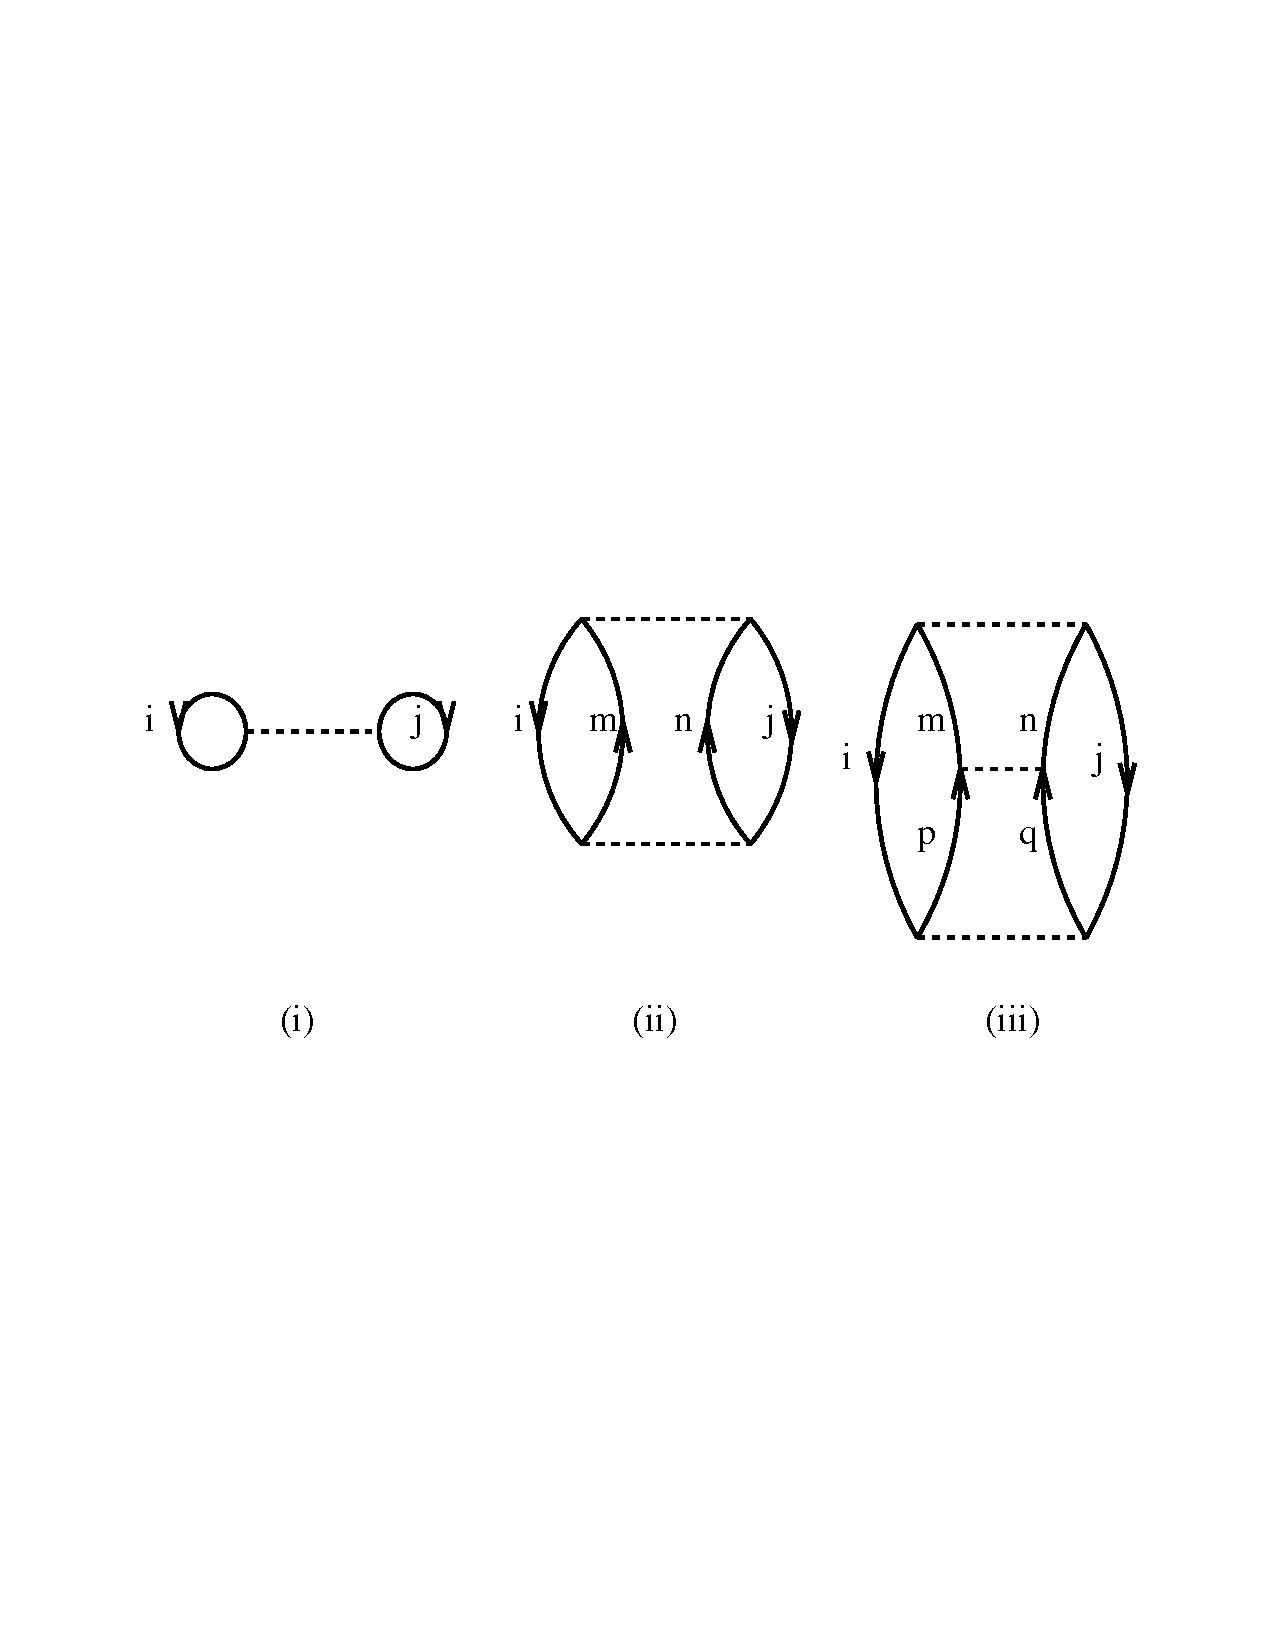
\includegraphics[width=0.6\linewidth]{fig-inf/goldstone.pdf}}
  \caption{
  Diagrams which enter the definition of the ground-state shift energy $\Delta E_0$. Diagram (i) is first order in the interaction $\hat{v}$, while diagrams (ii) and (iii) are examples of contributions to second and third order, respectively. \label{fig:goldstone}
  }
\end{figure}
%\clearpage % flush figures fig:goldstone


Using the standard diagram rules (see the discussion on coupled-cluster theory and many-body perturbation theory), the various
diagrams contained in the above figure can be readily calculated (in an uncoupled scheme)
\begin{equation}
   (i)=\frac{(-)^{n_h+n_l}}{2^{n_{ep}}}\sum_{ij\leq k_F}
       \langle ij\vert\hat{v}\vert ij\rangle_{AS},
\end{equation}
with $n_h=n_l=2$ and $n_{ep}=1$. As discussed  in connection with the diagram rules in the many-body perturbation theory chapter, $n_h$
denotes the number of hole lines, $n_l$ the number of closed
fermion loops and $n_{ep}$ is the number of so-called
equivalent pairs.
The factor $1/2^{n_{ep}}$ is needed since we want to count a pair 
of particles only once. We will carry this factor $1/2$ with us
in the equations below. 
The subscript $AS$ denotes the antisymmetrized and normalized matrix element
\begin{equation}
     \langle ij\vert\hat{v}\vert ij\rangle_{AS}=\langle ij \vert\hat{v}\vert ij\rangle-
     \langle ji \vert\hat{v}\vert ij\rangle.
\end{equation}
Similarly, diagrams (ii) and (iii) read
\begin{equation}
   (ii)=\frac{(-)^{2+2}}{2^2}\sum_{ij\leq k_F}\sum_{ab>k_F}
   \frac{\langle ij\vert\hat{v}\vert ab\rangle_{AS}
   \langle ab\vert\hat{v}\vert ij\rangle_{AS}}
   {\varepsilon_i+\varepsilon_j-\varepsilon_a-\varepsilon_b},
\end{equation}
and
\begin{equation}
   (iii)=\frac{(-)^{2+2}}{2^3}\sum_{k_i,k_j\leq k_F}\sum_{abcdk_F}
   \frac{\langle ij\vert\hat{v}\vert ab\rangle_{AS}
   \langle ab\vert\hat{v}\vert cd\rangle_{AS}
   \langle cd\vert\hat{v}\vert ij\rangle_{AS}}
   {(\varepsilon_i+\varepsilon_j-\varepsilon_a-\varepsilon_b)
   (\varepsilon_i+\varepsilon_j-\varepsilon_c-\varepsilon_d)}.
\end{equation}
In the above, $\varepsilon$ denotes the sp energies defined by
$H_0$.
The steps leading to the above expressions for the various
diagrams are rather straightforward. Though, if we wish to compute the
matrix elements for the interaction $v$, a serious problem
arises. Typically, the matrix elements will contain a term
(see the next section for the formal details) $V(|{\mathbf r}|)$, which
represents the interaction potential $V$ between two nucleons, where
${\mathbf r}$ is the internucleon distance.
All modern models
for $V$ have a strong short-range repulsive core. Hence,
matrix elements involving $V(|{\mathbf r}|)$, will result in large
(or infinitely large for a potential with a hard core)
and repulsive contributions to the ground-state energy. Thus, the
diagrammatic expansion for the ground-state energy in terms of the
potential $V(|{\mathbf r}|)$ becomes meaningless.

One possible solution to  this problem is provided by the well-known
Brueckner theory or the Brueckner $G$-matrix, or just the
$G$-matrix. In fact, the $G$-matrix is an almost indispensable
tool in almost every microscopic nuclear structure
calculation. Its main idea may be paraphrased as follows.
Suppose we want to calculate the function $f(x)=x/(1+x)$. If
$x$ is small, we may expand the function $f(x)$ as a power series
$x+x^2+x^3+\dots$ and it may be adequate to just calculate the first
few terms. In other words, $f(x)$ may be calculated using a low-order
perturbation method. But if $x$ is large
(or infinitely large), the above
power series is obviously meaningless.
However, the exact function
$x/(1+x)$ is still well defined in the limit
of $x$ becoming very large.

These arguments suggest that one should sum up the diagrams
(i), (ii), (iii) in fig.~\ref{fig:goldstone} and the similar ones
to all orders, instead of computing them one by one. Denoting this
all-order sum as $1/2\tilde{G}_{ijij}$, where we have
introduced the shorthand notation
$\tilde{G}_{ijij}=\langle k_ik_j\vert \tilde{G}\vert k_ik_j\rangle_{AS}$
(and similarly for $\tilde{v}$),
we have that
\begin{align}
      \frac{1}{2}\tilde{G}_{ijij}=&\frac{1}{2}\hat{v}_{ijij}
      +\sum_{ab>k_F}\frac{1}{2}\hat{v}_{ijab}\frac{1}{\varepsilon_i+\varepsilon_j-\varepsilon_a-\varepsilon_b}
      \nonumber \\
      & \times\left[\frac{1}{2}\hat{v}_{abij}+\sum_{cd>k_F}
      \frac{1}{2}\hat{v}_{abcd}\frac{1}
      {\varepsilon_i+\varepsilon_j-\varepsilon_c-\varepsilon_d}
      \frac{1}{2}V_{cdij}+\dots  \right].
\end{align}
The factor $1/2$ is the same as that discussed above, namely we want 
to count a pair of particles only once.
The quantity inside the brackets is just
$1/2\tilde{G}_{mnij}$ and the above equation can be
rewritten as an integral equation
\begin{equation}
      \tilde{G}_{ijij}=\tilde{V}_{ijij}
      +\sum_{ab>F}\frac{1}{2}\hat{v}_{ijab}\frac{1}{\varepsilon_i+\varepsilon_j-\varepsilon_a-\varepsilon_b}
      \tilde{G}_{abij}.
\end{equation}
Note that $\tilde{G}$ is the antisymmetrized $G$-matrix since
the potential $\tilde{v}$ is also antisymmetrized. This means that
$\tilde{G}$ obeys
\begin{equation}
  \tilde{G}_{ijij}=-\tilde{G}_{jiij}=-\tilde{G}_{ijji}.
\end{equation}
The $\tilde{G}$-matrix  is defined as
\begin{equation}
    \tilde{G}_{ijij}=G_{ijij}-G_{jiij},
\end{equation}
and the equation for $G$ is
\begin{equation}
      G_{ijij}=V_{ijij}
      +\sum_{ab>k_F}V_{ijab}\frac{1}
      {\varepsilon_i+\varepsilon_j-\varepsilon_a-\varepsilon_b}
      G_{abij},
      \label{eq:ggeneral}
\end{equation}
which is the familiar $G$-matrix equation. The above
matrix is specifically designed to treat a class of diagrams
contained in $\Delta E_0$, of which typical contributions
were shown in fig.~\ref{fig:goldstone}. In fact the sum of the diagrams
in fig.~\ref{fig:goldstone} is equal to $1/2(G_{ijij}-G_{jiij})$.

Let us now define a more general $G$-matrix as
\begin{equation}
      G_{ijij}=V_{ijij}
      +\sum_{mn>0}V_{ijmn}\frac{Q(mn)}
      {\omega -\varepsilon_m-\varepsilon_n}
      G_{mnij},
      \label{eq:gwithq}
\end{equation}
which is an extension of Eq. (\ref{eq:ggeneral}). Note that 
Eq. (\ref{eq:ggeneral}) has
$\varepsilon_i+\varepsilon_j$ in the energy denominator, whereas
in the latter equation we have a general energy variable $\omega$
in the denominator. Furthermore, in Eq. (\ref{eq:ggeneral})
we have a restricted
sum over $mn$, while in Eq. (\ref{eq:gwithq})
we sum over all $ab$ and we have
introduced a weighting factor $Q(ab)$. In Eq. (\ref{eq:gwithq}) $Q(ab)$
corresponds to the choice
\begin{equation}
   Q(a , b ) =
    \left\{\begin{array}{cc}1,&min(a ,b ) > k_F\\
    0,&\mathrm{else}.\end{array}\right. ,
\end{equation}
where $Q(ab)$ is usually referred to as the $G$-matrix Pauli
exclusion operator. The role of $Q$ is to enforce a selection
of the intermediate states allowed in the $G$-matrix equation. The above
$Q$ requires that the intermediate particles $a$ and $b$
must be both above the Fermi surface defined by $F$. We may enforce
a different requirement by using a summation over intermediate states
different from that in Eq. (\ref{eq:gwithq}).
An example is the Pauli operator
for the model-space Brueckner-Hartree-Fock method discussed below.


Before ending this section, let us rewrite the $G$-matrix equation
in a more compact form.
The sp energies $\varepsilon$ and wave functions are defined
by the unperturbed hamiltonian $H_0$ as
\begin{equation}
   H_0\vert \psi_a\psi_b=(\varepsilon_a+\varepsilon_b)
   \vert \psi_a\psi_b.
\end{equation}
The $G$-matrix equation can then be rewritten in the following
compact form
\begin{equation}
   G(\omega )=V+V\frac{\hat{Q}}{\omega -H_0}G(\omega ),
\end{equation}
with
$\hat{Q}=\sum_{ab}\vert \psi_a\psi_b\langle\langle \psi_a\psi_b\vert$.
In terms of diagrams, $G$ corresponds to an all-order sum of the
"ladder-type" interactions between two particles with the
intermediate states restricted by $Q$.

The $G$-matrix equation has a very simple form. But its
calculation is rather complicated, particularly for finite
nuclear systems such as the nucleus $^{18}$O. There are a
number of complexities. To mention a few, the Pauli operator
$Q$ may not commute with the unperturbed hamiltonian
$H_0$ and we have to make the replacement
\[
\frac{Q}{\omega -H_0}\rightarrow Q\frac{1}{\omega -QH_0Q}Q.
\]
The determination of the starting energy $\omega$ is also another
problem. 


In a medium such as nuclear 
matter we must account
for the fact that certain states are not available as intermediate
states in the calculation of the $G$-matrix.
Following the discussion above
this is achieved by introducing the medium
dependent Pauli operator $Q$. Further, the
energy $\omega$ of the incoming particles, given by a pure kinetic
term in a scattering problem between two unbound particles (for example two colliding protons), must be modified so as to allow
for medium corrections.
How to evaluate the Pauli operator for
nuclear matter is, however, not straightforward.
Before discussing how to evaluate the Pauli operator for nuclear matter,
we note that the $G$-matrix
is conventionally given in terms of partial waves and
the coordinates of the relative and center-of-mass motion.
If we assume that the $G$-matrix is diagonal in $\alpha$ ($\alpha$ is a shorthand
notation for $J$, $S$, $L$ and $T$), we  write the equation for the $G$-matrix as a 
coupled-channels equation in the relative and center-of-mass system
\begin{equation}
   G_{ll'}^{\alpha}(kk'K\omega )=V_{ll'}^{\alpha}(kk')
   +\sum_{l''}\int \frac{d^3 q}{(2\pi )^3}V_{ll''}^{\alpha}(kq)
   \frac{Q(q,K)}{\omega -H_0}
   G_{l''l'}^{\alpha}(qk'K\omega).
   \label{eq:gnonrel}
\end{equation}
This equation is similar in structure to the scattering
equations discussed in connection with nuclear forces (see the chapter on models for nuclear forces), except that we now have
introduced the Pauli operator $Q$ and a medium dependent two-particle
energy $\omega$. The notations in this equation follow those of the chapter on nuclear forces
where we discuss the solution of the scattering
matrix $T$.
The numerical details on how to solve the above $G$-matrix
equation through matrix inversion techniques are discussed below
Note however that the $G$-matrix may not be diagonal in $\alpha$.
This is due to the fact that the
Pauli operator $Q$ is not diagonal
in the above representation in the relative and center-of-mass
system. The Pauli operator depends on the
angle between the relative momentum and the center of mass momentum.
This angle dependence causes $Q$ to couple states with different
relative angular
momentua ${\cal J}$, rendering  a partial wave decomposition of the $G$-matrix equation 
rather difficult.
The angle dependence of the Pauli operator
can be eliminated by introducing the angle-average
Pauli operator, where one replaces the exact Pauli operator $Q$
by its average $\bar{Q}$ over all angles for fixed relative and center-of-mass
momenta.
The choice of Pauli operator is decisive to the determination of the
sp
spectrum. Basically, to first order in the reaction matrix $G$,
there are three commonly used sp spectra, all
defined by the solution of the following equations
\begin{equation}
   \varepsilon_{m} = \varepsilon (k_{m})= t_{m} + u_{m}=\frac{k_{m}^2}{2M_N}+u_{m},
   \label{eq:spnrel}
\end{equation}
and
\begin{align}
   u_{m} =& {\displaystyle \sum_{h \leq k_F}}\left\langle m h \right| G(\omega = \varepsilon_{m} + \varepsilon_h )
   \left| m h \right\rangle_{AS}  \hspace{3mm}k_m \leq k_M,  \\ \\
   u_m=&0, k_m > k_M.
   \label{eq:selfcon}
\end{equation}
For notational economy, we set $|{\bf k}_m|=k_m$.
Here we employ antisymmetrized matrix elements (AS), and $k_M$ is a cutoff
on the momentum. Further, $t_m$ is the sp kinetic
energy and similarly $u_m$
is the
sp potential.
The choice of cutoff $k_M$ is actually what determines the three
commonly used sp spectra.
In the conventional BHF approach one employs $k_M = k_F$,
which leads
to a Pauli operator $Q_{\mathrm{BHF}}$ (in the laboratory system) given by
\begin{equation}
   Q_{\mathrm{BHF}}(k_m , k_n ) =
    \left\{\begin{array}{cc}1,&min(k_m ,k_n ) > k_F\\
    0,&\mathrm{else}.\end{array}\right.
    \label{eq:bhf},
\end{equation}
or, since we will define an
angle-average Pauli operator in the relative and center-of-mass
system, we have
\begin{equation}
     \bar{Q}_{\mathrm{BHF}}(k,K)=\left\{\begin{array}{cc}
         0,&k\leq \sqrt{k_{F}^{2}-K^2/4}\\
         1,&k\geq k_F + K/2\\
	\frac{K^2/4+k^2 -k_{F}^2}{kK}&\mathrm{else},\end{array}\right.
    \label{eq:qbhf}
\end{equation}
with $k_F$ the momentum at the Fermi surface.

The BHF choice sets $u_k = 0$ for $k > k_F$, which leads
to an unphysical, large gap at the Fermi surface, typically
of the order of $50-60$ MeV. 
To overcome the gap
problem, Mahaux and collaborators 
introduced a continuous sp spectrum
for all values of $k$. The divergencies
which then may occur in Eq. (\ref{eq:gnonrel}) are taken care of by
introducing
a principal value integration in Eq. (\ref{eq:gnonrel}),
to retain only the
real part contribution to the $G$-matrix.


To define the energy denominators we will also make use of the
angle-average approximation.
The angle dependence is handled by the
so-called effective mass approximation. The single-particle energies
in nuclear matter are assumed to have the simple quadratic form
\begin{equation}
   \begin{array}{ccc}
   \varepsilon (k_m)=&
   {\displaystyle\frac{\hbar^{2}k_m^2}
   {2M_{N}^{*}}}+\Delta ,&\hspace{3mm}k_m\leq k_F\\
   &&\\
   =&{\displaystyle\frac{\hbar^{2}
   k_m^2}{2M_{N}}},&\hspace{3mm}k_m> k_F ,\\
   \end{array}
   \label{eq:spen}
\end{equation}
where $M_{N}^{*}$ is the effective mass of the nucleon and $M_{N}$ is the
bare nucleon mass. For particle states above the Fermi sea we choose
a pure kinetic energy term, whereas for hole states,
the terms $M_{N}^{*}$ and $\Delta$, the latter being 
an effective single-particle
potential related to the $G$-matrix, are obtained through the
self-consistent Brueckner-Hartree-Fock procedure.
The sp potential is obtained through the same angle-average approximation
\begin{align}
  \label{eq:Uav}
   U(k_m) & =\sum_{l\alpha} (2T+1)(2J+1)
   \left \{ \frac{8}{\pi}\int_{0}^{(k_F-k_m)/2}
   k^2dk G_{ll}^{\alpha}(k,\bar{K}_1) \right.  \\
   &    \left.
    + \frac{1}{\pi k_m}\int_{(k_F-k_m)/2}^{(k_F+k_m)/2}
   kdk (k_F ^2-(k_m-2k)^2)
   G_{ll}^{\alpha}(k,\bar{K}_2)  \right \}  \nonumber,
\end{align}
where we have defined
\begin{equation}
    \bar{K}_1^2=4(k_m^2+k^2),
\end{equation}
and
\begin{equation}
    \bar{K}_2^2=4(k_m^2+k^2)-(2k+k_m-k_F)(2k+k_1+k_F).
\end{equation}
This
self-consistency scheme consists in choosing adequate initial values of the
effective mass and $\Delta$. The obtained $G$-matrix is in turn used to
obtain new values for $M_{N}^{*}$ and $\Delta$. This procedure
continues until these parameters vary little.





% ------------------- end of main content ---------------


% #ifdef PREAMBLE
\printindex

\end{document}
% #endif

